% Created 2023-08-27 Sun 13:47
% Intended LaTeX compiler: pdflatex
\documentclass[ee,msthesis]{usuthesis}
\usepackage[utf8]{inputenc}
\usepackage[T1]{fontenc}
\usepackage{graphicx}
\usepackage{longtable}
\usepackage{wrapfig}
\usepackage{rotating}
\usepackage[normalem]{ulem}
\usepackage{amsmath}
\usepackage{amssymb}
\usepackage{capt-of}
\usepackage{hyperref}
\usepackage{amsmath}                         % Miscellaneous enhancements for mathematics
\usepackage{amssymb}                         % Math symbols
\usepackage{algorithm2e}                    % Algorithms
\usepackage{amsfonts}                       % Cool math fonts
\usepackage{booktabs}                       % Used for lines in table
\usepackage{lipsum}                         % Dummy filler text
\usepackage{multicol}                       % Add capability to make columns
\usepackage{multirow}                       % Add capability to make rows
\usepackage{pgfgantt}                       % Add capability to create gantt charts
\usepackage{standalone}                     % Allow standalone documents
\usepackage{subcaption}                     % Allow subfigures
\usepackage{subfloat}                       % Subfigures
\usepackage{tabularx}                        % Add more contol to tables
\usepackage{listings}                       % Display code
\usepackage{doi}                            % Hyperling DOI
\usepackage{hyperref}                       % Cool clean hyperlinks
\setlength\parindent{0pt}                   % No indent for paragraphs
\usetikzlibrary{arrows.meta}                % Arrows for tikz
\renewcommand*{\chapterautorefname}{Chapter}
\renewcommand*{\sectionautorefname}{Section}
\renewcommand*{\subsectionautorefname}{Subsection}
\renewcommand*{\subsubsectionautorefname}{Subsubsection}
\renewcommand*{\paragraphautorefname}{Paragraph}
\renewcommand*{\algorithmautorefname}{Algorithm}
\newcommand{\Or}{\textbf{ or }}
\renewcommand*{\And}{\textbf{ and }}
\newcommand\mycommfont[1]{\footnotesize\ttfamily\textcolor{gray}{#1}}
\newcommand{\T}{\mathcal{T}}                % To make it clear the difference
\newcommand{\Tau}{T}                        % between Tau and T
\newcommand{\AC}{AC(u, d, v, \eta)}            % Set the parameters for AC once
\newcommand{\PC}{PC(u, d, v)}               % Set the parameters for PC once
\newcommand{\ACi}{AC(u_i, d_i, v_i, \eta_i)}% Set the parameters for AC once
\newcommand{\PCi}{PC(u_i, d_i, v_i)}        % Set the parameters for PC once
\newcommand{\Not}{\textbf{not }}            % Custom `not' operator
\newcommand{\visit}{(b_i, a_i, e_i, u_i, d_i, v_i, \eta_i, \xi_i)}
\newcommand{\I}{\mathbb{I}}                 % Set of visit tuples
\newcommand{\C}{\mathbb{C}}                 % Charger availability information
\newcommand{\U}{\mathcal{U}}                % Uniform distribution
\newcommand{\Sol}{\mathbb{S}}               % A shorthand for visit tuple
\newcommand{\M}{\mathbb{M}}                 % A shorthand for the metadata
\newcommand{\Hd}{\mathbb{H}}                % Set of discrete times
\newcommand{\Nu}{\mathcal{V}}               % Draw a nice Nu
\newcommand{\Iset}{\mathcal{I}}             % Set of visits 1-I
\newcommand{\Isetinit}{\mathcal{I}_0}       % Set of visits inital visits
\newcommand{\Isetfinal}{\mathcal{I}_f}      % Set of visits final visits
\newcommand{\Bset}{\mathcal{B}}             % Set of visits 1-B
\newcommand{\Qset}{\mathcal{Q}}             % Set of visits 1-Q
\newcommand{\Jset}{\mathcal{J}}             % Set of visits 1-J
\newcommand{\Jsetq}{\mathbb{J}}             % Set of visits 1-J for queue active times
\newcommand{\Hset}{\mathcal{H}}             % Set of visits 1-H
% The Committee
\majorprof{Dr. Droge, Ph.D.}
\firstreader{Robert L. Forward, Ph.D.}
\secondreader{Albert Einstein, Ph.D.}
\thirdreader{Gottfried Liebniz, Ph.D.}

% Graduate Dean
\graddean{ D. Richard Cutler, Ph.D.}
\deantitle{ Vice Provost of Graduate Studies}

% Degree Information
\degree{Master of Science}
\month{Dec}
\gradyear{2023}
\newtheorem{definition}{Definition}[section]
\author{Alexander Brown}
\date{}
\title{The Simulated Annealing Fully Fuzzy Position Allocation Problem Utilizing Mixed Integer Linear Programming Constraints with Non-Linear Battery Dynamics}
\hypersetup{
 pdfauthor={Alexander Brown},
 pdftitle={The Simulated Annealing Fully Fuzzy Position Allocation Problem Utilizing Mixed Integer Linear Programming Constraints with Non-Linear Battery Dynamics},
 pdfkeywords={},
 pdfsubject={},
 pdfcreator={Emacs 29.1 (Org mode 9.6.7)}, 
 pdflang={English}}
\begin{document}

\maketitle
\let\ref\autoref                            % Redifine `\ref` as `\autoref` because lazy
\SetCommentSty{mycommfont}                  % Set the comment color

\tableofcontents
\listoftables
\listoffigures

\let\ref\autoref                            % Redifine `\ref` as `\autoref` because lazy

\body  % set main body style

\chapter{INTRODUCTION}
\label{sec:introduction}
Public transportation system are crucial in any urban area; however, the increased awareness and concern of
environmental impacts of petroleum based public transportation has driven an effort to reduce the pollutant footprint
\cite{de-2014-simul-elect,xylia-2018-role-charg,guida-2017-zeeus-repor-europ,li-2016-batter-elect}. Particularly,
the electrification of public bus transportation via battery power, i.e., battery electric buses (BEBs), has received
significant attention \cite{li-2016-batter-elect}. Although the technology provides benefits beyond reduction in
emissions, such as lower driving costs, lower maintenance costs, and reduced vehicle noise, battery powered systems
introduce new challenges such as larger upfront costs, and potentially several hours long ``refueling'' periods
\cite{xylia-2018-role-charg,li-2016-batter-elect}. Furthermore, the problem is exacerbated by the constraints of the
transit schedule to which the fleet must adhere, the limited amount of chargers available, and the adverse affects in
the health of the battery due to fast charging \cite{lutsey-2019-updat-elect}.

Many recent efforts have been made to simultaneously solve the problems of route scheduling, and charging fleets and
determining the infrastructure upon which they rely, e.g., \cite{wei-2018-optim-spatio,sebastiani-2016-evaluat-elect,hoke-2014-accoun-lithium,wang-2017-elect-vehic}. Several simplifications are made to make these problems
computationally feasible. These simplifications to the charge scheduling model include utilizing only fast chargers
while planning \cite{wei-2018-optim-spatio,sebastiani-2016-evaluat-elect,wang-2017-optim-rechar,zhou-2020-bi-objec,yang-2018-charg-sched,wang-2017-elect-vehic,qin-2016-numer-analy,liu-2020-batter-elect}. If slow chargers are used,
they are only employed at the depot and not the station \cite{he-2020-optim-charg,tang-2019-robus-sched}. Some
approaches also simplify by assuming a full charge is always achieved
\cite{wei-2018-optim-spatio,wang-2017-elect-vehic,zhou-2020-bi-objec,wang-2017-optim-rechar}. Others have assumed
that the charge received is proportional to the time spent on the charger
\cite{liu-2020-batter-elect,yang-2018-charg-sched}, which can be a valid assumption when the battery state-of-charge
(SOC) is below 80\% charge \cite{liu-2020-batter-elect}.

The proposed work presented here intends to extend the work of the PAP's novel approach to BEB charger scheduling even
further. The PAP's reenvisioning of the BAP provides the stepping stones on which to further extend the utility of this
robust technology. The intended work to be introduced, much of which has been completed, promises much potential for
further research and development in regard to BEBs. What follows is a proposal for a Simulated Annealing (SA)
implementation of the PAP utilizing Fully Fuzzy Mixed Integer Linear Programming (FFMILP) constraints with non-linear
battery dynamics.

\section{Background and Related Work}
\label{sec:background-and-related-work}
The charging problem is a problem that has been of increasing interest and therefore also increasing in relevancy in the
EV/BEB industry. It is thus important to address the state of the art by introducing relevant problems in BEB
scheduling. The areas of interest will then be detailed to the work proposed in this work, the Berth Allocation Problem
(BAP) and the Position Allocation Problem (PAP).

\subsection{Problem Description}
\label{sec:problem-description}
It is assumed that there are a total of \(I\) visits to the station by \(B\) buses. There are a total of \(Q\) queues for the
bus at the station. Let \(\mathcal{Z}\) be the set of integers, given a set of bus arrivals to a charging station \(i \in \{1,..., I\}
= \Iset \subset \mathcal{Z}\) with a set of chargers to be queued \(q \in \{1,..., Q\} = \Qset \subset \mathcal{Z}\) where the bus is indicated by an
identification number \(b \in \{1,..., B\} = \Bset \subset \mathcal{Z}\). Each bus arrival, \(i\), can be represented by the tuple: \(\visit\),
in which the ordered elements denote the bus identification number, \(b_i\), arrival time to the station, \(a_i\), departure
time from the station, \(e_i\), time to start charging, \(u_i\), time to stop charging, \(d_i\), the charger queue for the bus
to be placed into, \(v_i\), and the initial State Of Charge (SOC), \(\eta_i\).

It is assumed that each visit occurs over the time horizon \(T = \{t : t_0 \le t \le t_f \}\). The set of all arrivals is
represented by the set \(\I = \{\forall i \in \Iset \; \visit: b_i, \xi_i \in \Bset, a_i, e_i, u_i, d_i \in T, v_i \in \Qset \}\). The
concept of ``arrivals'' is derived from the PAP \cite{qarebagh-2019-optim-sched}. This idea of arrivals is useful in the
sense that it is easy to describe the state of any arbitrary arrival; however, although a bus may revisit the station
multiple times, the model assumes that each arrival is unique (i.e. no two bus arrives twice) therefore a system must be
put in place to track each bus over each arrival. That is why a bus identifier is placed in the tuple, and in that way
each bus can be tracked over each arrival.

For each arrival a bus must be placed in a singular queue, \(v_i \in \Qset\). The charger \(q\) is assumed to be either a fast
or slow charger or no charger at all. A bus is only allowed to visit one queue per visit; however, there may be multiple
buses charging simultaneously. The amount of time the bus is allowed to charge is dictated by the scheduled arrival time
and required departure time, \([a_i, e_i]\). Although a bus must be placed in a queue, if a bus does not require much
charge, or none at all, partial charges, or no charging, is allowed. It is not allowed for the bus to charge over its
battery capacity limit. The battery charging rate is modeled as linear, which remains accurate up to about an SOC of 80\%
charge \cite{li-2016-batter-elect}.

Each bus arrival, except for the last arrival for each bus, has a paired ``route'' that the bus must perform. This route,
as one would expect, causes the bus to discharge by some certain amount. This paper assumes an average discharge over a
period of in which an estimated discharge is calculated for each route, \(\Delta_i\). The charge supplied while at the station
is required to supply enough charge for each route with an additional battery capacity percentage, \(m\), acting as a
safety factor.

The scheduler's task shall be to schedule the set of arrivals \(\I\) to fulfill the minimum charge requirements over the
time horizon \(T\) as well as minimize the demand cost and consumption cost. The objective function and constraints are
discussed in further detail in section \ref{sec:objective-function}.

\subsection{State Of The Art}
\label{sec:orgc280663}
The intent of the proposed work is to build upon the Position Allocation Problem \cite{qarebagh-2019-optim-sched}, a
modification of the well studied Berth Allocation Problem (BAP), as a means to schedule the charging of electric
vehicles \cite{buhrkal-2011-model-discr,frojan-2015-contin-berth,imai-2001-dynam-berth}. The BAP model is a rectangle
packing problem with the goal of allocating space for incoming vessels to be berthed and serviced as depicted in
\autoref{subfig:bapexample}. The BAP can be modeled continuously and discretely both temporally and spatially
\cite{buhrkal-2011-model-discr,frojan-2015-contin-berth}. Furthermore, the demand to efficiently handle an
ever-growing demand for servicing cargo, with an estimated 1.24 billion of the 8.02 billion tonnes of all shipping cargo
in 2007 \cite{buhrkal-2011-model-discr}, implies a need for well planned berthing, which in turn provides a strong pool
of robust literature to draw from. Methods of handling multiple quays to handle general berthing scenarios
\cite{frojan-2015-contin-berth,dai-2008-suppl-chain-analy}, heuristic procedures for quicker solve times have been
introduced \cite{imai-2001-dynam-berth}, static (full time horizon) and dynamic (rolling-time horizon) models have been
created for daily and real-time solutions, respectively, and even fuzzy set theory has been applied to allow for more
flexible schedules \cite{bello-2019-fuzzy-activ}. An example of a standard BAP solution is visualized in
\autoref{fig:bap}. The x and y-axis represent time and berthing space, respectively. The figure discretizes the berthing
space, but it may be continuous if desired. The shaded rectangles' widths represent their respective allocated service
times, and their heights represent the physical space taken by each vessel.

The PAP provides a basis for assigning BEBs to queues in order to be charged. Let's begin by defining some of the
assumptions made by the PAP. Each arriving vessel requires both time and space to be serviced and thus must be carefully
assigned a berthing location \cite{imai-2001-dynam-berth}. Vessels are lined up parallel to the berth to be serviced
and are horizontally queued as shown in \autoref{subfig:bapexample}. The PAP utilizes this notion of queuing for
scheduling vehicles to be charged, as shown in \autoref{subfig:papexample}. The PAP is formulated as a rectangle packing
problem and assumes that vehicle charging will take a predefined amount of time, the quantity of vehicles that can
charge simultaneously is limited by the physical width of the vehicles and the charger length. It is assumed that each
vehicle visits the charger a single time \cite{qarebagh-2019-optim-sched}.

\begin{subfigures}
    %%~~~~~~~~~~~~~~~~~~~~~~~~~~~~~~~~~~~~~~~~~~~~~~~~~~~~~~~~~~~~~~~~~~~~~~~~~~~~
    % BAP
    \begin{figure}[htpb]
    \centering
        \includestandalone{sup-doc/milp-pap-paper-frontiers/img/bap}
        \caption{Example of berth allocation. Vessels are docked in berth locations (horizontal) and are queued over
          time (vertical). The vertical arrow represents the movement direction of queued vessels and the horizontal
          arrow represents the direction of departure.}
        \label{subfig:bapexample}
    \end{figure}
    \hfill

    %%~~~~~~~~~~~~~~~~~~~~~~~~~~~~~~~~~~~~~~~~~~~~~~~~~~~~~~~~~~~~~~~~~~~~~~~~~~~~
    % PAP
    \begin{figure}[htpb]
    \centering
        \includestandalone{sup-doc/milp-pap-paper-frontiers/img/pap}
        \caption{Example of position allocation. Vehicles are placed in queues to be charged and move in the direction
          indicated by the arrow.}
        \label{subfig:papexample}
    \end{figure}
\end{subfigures}

As stated previously, the proposed project will further improve upon the PAP. While there are many avenues that may be
taken, the first task is to adapt the PAP to accommodate a BEB charging scenario where a fleet of buses is prescribed a
set of routes that they must adhere to. Firstly, due to the unknown charge state that a bus may arrive in, the charge
time must be variable, rather than an input parameter as is done currently for the BAP and PAP. Furthermore, both the
BAP and PAP consider each arrival to be unique; thus, a method of tracking buses must be implemented. As for queuing,
the PAP models the set of chargers as one continuous line; thus, the set of chargers must be discretized. The last set
of additions made upon the PAP is the design of the objective function. Input parameters are selected in such a manner
as to minimize the number of fast and slow charger utilized as well as minimize the energy consumption. The result is a
MILP formulation that coordinates charging times and charger type for every visit that each bus makes to the station
while considering a proportional dynamic charging model with scheduling constraints. The described improvements have
been completed as a proof of concept in what is known as the MILP-PAP. This proof of concept was written in the Python
programming language using Gurobi as the MILP solver.

While the linear battery dynamics is a valid assumption when the battery State-Of-Charge (SOC) is below 80\%
\cite{liu-2020-batter-elect}, non-linear battery dynamics can be implemented to increase the accuracy of the model. A
common way to model the non-linear battery dynamics is utilizing CCCV \cite{abdollahi-2016-optim-batter,chen-2008-desig-grey}. \cite{zhang-2021-optim-elect} further suggests that the dynamics can be modeled as a piecewise
function containing a linear and non-linear component. Others have modeled the battery dynamics as a discrete first
order dynamics model \cite{whitaker-2022-a-network}. The first-order differential system, when provided a step input,
approximates the non-linear relationship between time and the current SOC \cite{whitaker-2022-a-network}. The
first-order differential method is method proposed to be pursued.

One of the drawbacks of the MILP implementation is the strict solution that is generated. Suppose that a solution was
generated, but due to weather conditions a bus arrives at the station five minutes late. The generated solution is no
longer valid due to one bus arriving late. This also could arise as an issue if a bus arrives early to the station. To
make matters worse, if a bus were to not adhere to the generated solution early on in the working day, the majority of
the solution is now void, and a new solution must be generated if optimality is desired. The crux of the problem is that
the time of arrival is uncertain. A potential solution to this problem is to fuzzify the MILP model.

Fuzzy mathematical programming is useful in situations where imprecise parameters exist \cite{bello-2019-fuzzy-activ}.
There are many methodologies that exist to solve Fully Fuzzy Linear Programs; however, the primary strategy of solving
FFLP problems is converting them into a classical (crisp) model
\cite{bello-2019-fuzzy-activ,nasseri-2013-fully,kaur-2016-introd-fuzzy}. The chosen technique to pursue is the Kumar
and Kaurs method \cite{kaur-2016-introd-fuzzy}. A model for the Fuzzy MILP-PAP has been drafted, but yet has been
implemented.

\subsection{Mixed Integer Linear Programming}
\label{sec:orgf00bd80}
A mixed integer linear programming (MILP) problem is a class of constrained optimization in which one seeks to find a
set of continuous or integer values that maximizes or minimizes an objective function while satisfying a set of
constraints \cite{chen-2010-applied}. Given a general objective function \(J\), decision variables (i.e. variables of
optimization) \(x_j \in \mathbb{R}\) and \(y_k \in \mathbb{Z}^+\), and input parameters \(c_j, d_k, a_{ij}, g_{ik}, b_i \in \mathbb{R}\), a MILP has the
mathematical structure represented in \ref{eq:milp-structure} \cite{chen-2010-applied}.

\begin{equation}
\label{eq:milp-structure}
\begin{array}{lll}
\text{max}   & J = \sum_j c_j x_j + \sum_k d_k y_k            &                 \\
\text{subject to} & \sum_j a_{ij} x_j + \sum_k g_{ik} y_k  \le b_i & (i = 1,2,...,m) \\
                  & x_j \ge 0                                      & (j = 1,2,...,n) \\
                  & y_k \in \mathbb{Z^+}0                          & (k = 1,2,...,n) \\
\end{array}
\end{equation}

This formulation of the MILP is also referred to as ``crisp''. By this it is meant that each variable in the formulation
acts as an injective mapping to its number representation. In other words, every variable has a one-to-one mapping from
variable to value \cite{kaur-2016-introd-fuzzy}.

\subsection{Overview of the BAP}
\label{sec:overview-of-the-bap}
\begin{figure}
  \centering
  \includegraphics{sup-doc/milp-pap-paper-frontiers/img/spatiotemporal-packing}
  \caption{Example of rectangle packing problem.}
  \label{fig:packexample}
\end{figure}

The BAP is a rectangle packing problem where a set of rectangles, \(\mathbb{O}\), are attempted to be optimally placed in
a larger rectangle, \(O\), as shown in \autoref{fig:packexample}. The rectangle packing problem is an NP-hard problem that
can be used to describe many real life problems \cite{bruin-2013-rectan-packin,murata-1995-rectan}. In some of these
problems, the dimensions of \(\mathbb{O}\) are held constant such as in the problem of packing modules on a chip, where
the widths and height of the rectangles represent the physical width and heights of the modules
\cite{murata-1995-rectan}. Other problems, such as the BAP can allow one side of the rectangle to vary depending on its
assigned position (e.g. the varying lengths of the vessels) \cite{buhrkal-2011-model-discr}.

The BAP solves the problem of optimally assigning incoming vessels to berth positions to be serviced
(\autoref{subfig:bapexample}). The width and height of \(O\) time horizon \(T\) and represent the berth length \(S\),
respectively. Similarly, the width and height for \(\mathbb{O}\) represent the time spent to service vessel \(i\) and the
space taken by docking vessel \(i\), respectively. In the BAP, the vessel characteristics (length of the vessel, arrival
time, handling time, desired departure time) are assumed to be known for all vessels to be serviced. A representation of
a BAP solution is shown in \autoref{fig:bap}. The x and y-axis represent time and space, respectively. The grey squares,
labeled A, B, C, and D, represent berthed vessels. The width of the boxes represent the time spent being serviced, and
the height represents the amount of space the vessel requires on the berth. The vertical line adjacent
 ``Arrival Time'' represents the actual
time that the vessel arrives and is available to be berthed. ``Berthing Time'' is the time the vessel is berthed and
begins being serviced. ``Completion time'' represents the time at which the berthing space becomes available again.
\chapter{OBJECTIVES}
\label{sec:objectives}
The field of BEB and EV research provides exciting many avenues and is continuing to gain traction in industry as BEBs
and EVs replace their gasoline counterparts. The identified concentration of study stated in this work is to provide a
novel approach based on the well studied BAP problem that provides a robust charging schedule for BEBs that minimizes
monetary costs for the user. The objectives proposed for the BEB charging plan research includes what follows.

\section{Mathematically model the PAP to optimally assign BEBs to station with unknown charging times}
\label{sec:org9853aae}
The PAP, as previously described, was designed for a predefined stream of EVs with a known SOC upon arrival, much like
how the BAP is formulated. This modeling does not align with the BEBs for the following reasons and must be addressed:

\begin{enumerate}
\item Each arrival is modeled as a unique visit which is not how buses operate. The BEBs repeatedly visit the same stops,
including the bus station where it is assumed they will be charged. The BEB must be given a unique identifier such
that its SOC may be tracked over its many visits and even for the obvious reason of being able to identify and
prescribe a BEB to their defined charging schedule.

\item As alluded in the previous action, the method of tracking the SOC is also of interest so that the charging schedule
provided does not result in undercharged BEBs being sent underway to perform their route, or on the opposite side, be
over-charged. Furthermore, it is assumed that the BEBs initial SOC will be known at the beginning of the day, but the
initial SOCs for subsequent visits will be known, and thus must be dynamically calculated. For accuracy of the SOC of
the BEB while charging, non-linear battery dynamics will be assumed.

\item The PAP models the charging station as a continuous bar, which is not favorable for the BEB model. It is of interest
to discretize the charging station to accommodate both slow and fast chargers. The slow chargers with be incentivized
whereas the fast chargers will be utilized only when required. This will be done for battery health
\cite{motapon-2020-gener-cycle}.
\end{enumerate}

Note that for this objective, all the actions described have been researched and implemented bar the non-linear
battery dynamics. The implementation of the above actions with linear battery dynamics will subsequently be referred to
as the MILP-PAP.

\section{Mathematically model the PAP to provide a robust solution}
\label{sec:obj-math-model-robust}
\begin{enumerate}
\item The MILP-PAP addresses the problem of specifying a lower bound for the BEBs when creating a charging schedule. A
problem arises when the lower bound specified does not allow for a solution to be generated because the minimum SOC
percentage constraint has been violated. It is proposed to introduce a penalty method for the lower bound in an
attempt to relax the constraint and create a larger solution space.

\item One of the drawbacks of the MILP implementation is the strict solution that is generated. Suppose that a solution was
generated, but due to weather conditions a bus arrives at the station five minutes late. The generated solution is no
longer valid due to one bus arriving late. This also could arise as an issue if a bus arrives early to the station.
To make matters worse, if a bus were to not adhere to the generated solution early on in the working day, the
majority of the solution is now void, and a new solution must be generated if optimality is desired. The crux of the
problem is that the time of arrival is uncertain. A solution to this problem is to fuzzify the MILP model.
\end{enumerate}

\section{Minimize the monetary cost of charging the BEBs}
\label{sec:orgc966771}

\begin{enumerate}
\item The previous objective mentioned the fact of favoring the use of slow chargers over fast chargers. This also results
in a reduction in monetary cost as it is cheaper in purchase and actively use slow chargers as they draw less
electricity \cite{he-2020-optim-charg}.

\item Another method of minimizing the monetary cost is to minimize the consumption cost. That is, minimize the total
amount of energy consumed by the system. Furthermore, the cost of electricity is not constant throughout the day,
thus it would be of interest to allow accommodations for peak hours of electricity use to more aggressively reduce
energy use.

\item Electricity companies also calculate energy use based on a value known as the peak 15. The peak 15 defines a method
of charging a base rate for electricity usage and adjusting based on power use. The power usage is monitored and averaged
over 15 minutes increments. If the average energy use exceeds a predefined threshold, the rate for electricity will
increase proportional to the new average. The cost is known as the demand cost and is of interest to minimize.
\end{enumerate}
\chapter{APPROACH}
\label{sec:proposed-project}
\section{Mathematically model the PAP to optimally assign BEBs to station with unknown charging times}
\label{sec:math-model-pap}
This section introduces the actions and formulations associated with the objective described in \ref{sec:objectives}. This
section addresses the actions by deriving a method of identifying buses for subsequent visits, utilizing that to
formulate a way of estimating the SOC during the BEBs charging phase. The method introduced in this section demonstrates
the linear battery dynamics that have been implemented in the MILP-PAP. Non-linear dynamics will then be introduced with
a brief description of the mathematical approach that will be taken. The derivation also demonstrates how the model will
discretize the queuing space to accommodate chargers of multiple varieties.

\subsection{The PAP Formulation}
\label{sec:input-variables}
The BAP forms the basis of the PAP; however, there are some differences in the way the variables are interpreted. For the
\(i^{th}\) visit, starting service time, \(u_i\), is now the starting charge time, the berth location, \(v_i\), is now the
charger queue for assignment, and the service time, \(s_i\), is now the elapsed charge time. There are also a few clarifying concepts
about how the system is modeled. The PAP models the set of chargers as one continuous line; that is, the natural
behavior of the PAP model is to allow vehicles to be queued anywhere along \([0,S]\). Similarly, the charge times are
continuous and can be placed anywhere on the time horizon, \([0,T]\), as long as the allocated times do not interfere with
other scheduled charge times. The PAP formulation's parameters can be divided into two categories: input parameters and
decision variables. Each type will now be introduced. The following parameters are constant inputs into the MILP.

\begin{itemize}
	\item $S$   : Size of the vehicle
	\item $T$   : time horizon
	\item $n_V$ : total number of incoming vehicles
	\item $s_i$ : charging time for vehicle $i;\; 1 \leq i \leq n_N$
	\item $s_i$ : width of vehicle $i;\; 1 \leq i \leq n_N$
	\item $a_i$ : arrival time of vehicle $i;\; 1 \leq i \leq n_N$
\end{itemize}

These constants define the problem bounds. The following list provides a series of decision variables used in the
formulation.

\begin{itemize}
    \item $u_i$    : starting charge time for vehicle $i;\; 1 \leq i \leq n_N$
    \item $v_i$    : assigned charge queue for vehicle $i;\; 1 \leq i \leq n_N$
    \item $d_i$    : departure time for vehicle $i;\; 1 \leq i \leq n_N$
    \item $\sigma_{ij}$ : binary variable that determines ordering of vehicles $i$ and $j$ in time
    \item $\psi_{ij}$ : binary variable that determines relative position of vehicles $i$ and $j$ when charging simultaneously
\end{itemize}

To determine the values for each of these decision variables, a MILP is formulated in \cite{qarebagh-2019-optim-sched}
and shown here for completeness.

\begin{equation}
	\label{eq:bapobjective}
	\min\; \sum_{i=1}^N (d_i - a_i)
\end{equation}

Subject to:
\begin{subequations}
\label{eq:bapconstrs}
\begin{align}
    u_j - u_i - s_i - (\sigma_{ij} - 1)T \geq 0                  \label{subeq:baptime}          \\
    v_j - v_i - s_i - (\psi_{ij} - 1)S \geq 0                \label{subeq:bapspace}           \\
    \sigma_{ij} + \sigma_{ji} + \psi_{ij} + \psi_{ji} \geq 1 \label{subeq:bapvalid_pos}     \\
    \sigma_{ij} + \sigma_{ji} \leq 1                              \label{subeq:bapsigma}        \\
    \psi_{ij} + \psi_{ji} \leq 1                              \label{subeq:bapdelta}        \\
    s_i + u_i = d_i                                               \label{subeq:bapdetach}       \\
    a_i \leq u_i \leq (T - s_i)                                   \label{subeq:bapvalid_starts} \\
    \sigma_{ij} \in \{0,1\},\;\psi_{ij} \in \{0,1\}\;           \label{subeq:bapsdspace}      \\
    v_i \in [0, S ]                                               \label{subeq:bapvspace}
\end{align}
\end{subequations}

\noindent

The objective function, \autoref{eq:bapobjective}, minimizes the time spent to service each vehicle by minimizing over
the sum of differences between the departure time, \(d_i\), and arrival time, \(a_i\). i.e., It seeks to get each vehicle
charged and on its way as quickly as possible.

\autoref{subeq:baptime}-\autoref{subeq:bapdelta} are used to ensure that individual rectangles do not overlap. For the
PAP, they ensure that two vehicles charging simultaneously are at different positions and, similarly, two vehicles that
have overlapping positions do not overlap temporally. \autoref{subeq:baptime} establishes temporal ordering when active
(\(\sigma_{ij}=1\)). Similarly, when \(\psi_{ij} =1\) in \autoref{subeq:bapspace} then spatial ordering is established. Constraints
\autoref{subeq:bapvalid_pos}-\autoref{subeq:bapdelta} enforce that spatial and/or temporal ordering is established
between each possible queue/vehicle pair. Constraints \autoref{subeq:bapsigma} and \autoref{subeq:bapdelta} enforce
consistency. For example, \autoref{subeq:bapsigma} enforces that vehicle \(i\) cannot come before vehicle \(j\) and vehicle
\(j\) simultaneously come before vehicle \(i\).

The last constraints force relationships between arrival time, charge start time, and departure time.
\autoref{subeq:bapdetach} states that the service start time, \(u_i\), plus the time to service vehicle \(i\), \(s_i\), must
equal the departure time, \(d_i\). \autoref{subeq:bapvalid_starts} enforces the arrival time, \(a_i\), to be less than or
equal to the service start time, \(u_i\), which in turn must be less than or equal to the latest time the vehicle may
begin to be serviced to stay within the time horizon. \autoref{subeq:bapsdspace} ensures that \(\sigma_{ij}\) and
\(\psi_{ij}\) are binary. \autoref{subeq:bapvspace} ensures that the assigned value of \(v_i\) is a valid charging position.
\begin{table}[!htpb]
  \caption{Notation used throughout the paper}
  \label{tab:variables}
  \centering
  \begin{tabularx}{\textwidth}{l l}
    \toprule
    \textbf{Variable} & \textbf{Description}                                                                               \\
    \toprule
    \multicolumn{2}{l}{Input values}                                                                                       \\
    $n_B$        & Number of buses                                                                                         \\
    $M$          & An arbitrary very large upper bound value                                                               \\
    $n_V$        & Number of total visits                                                                                  \\
    $n_Q$        & Number of queues                                                                                        \\
    $n_C$ 	 & Number of chargers                                                                                      \\
    $\mathbb{V}$ & Set of visit indices, $\mathbb{V} = \{1, ..., n_V\}$                                                    \\
    $\mathbb{B}$ & Set of bus indices, $\mathbb{B} = \{1, ..., n_B\}$                                                      \\
    $\mathbb{Q}$          & Set of queue indices, $\mathbb{Q} = \{1, ..., n_Q\}$                                                             \\
    $i,j$        & Indices used to refer to visits                                                                         \\
    $b$ 	 & Index used to refer to a bus                                                                            \\
    $q$ 	 & Index used to refer to a queue                                                                          \\
    \hline
    \multicolumn{2}{l}{Problem definition parameters}                                                                      \\
    $\Gamma$   & $\Gamma: \mathbb{V} \rightarrow \mathbb{B}$ with $\Gamma_i$ used to denote the bus for visit $i$                                   \\
    $\alpha_i$ & Initial charge percentage time for visit $i$                                                                   \\
    $\beta_i$ & Final charge percentage for bus $i$ at the end of the time horizon                                             \\
    $\epsilon_q$ & Cost of using charger $q$ per unit time                                                                        \\
    $\Upsilon$   & $\Upsilon: \mathbb{V} \rightarrow \mathbb{V}$ mapping a visit to the next visit by the same bus with $\Upsilon_i$ being the shorthand. \\
    $\kappa_b$ & Battery capacity for bus $b$                                                                                   \\
    $\Delta_i$ & Discharge of visit over route $i$                                                                              \\
    $\nu_b$ & Minimum charge allowed for bus $b$                                                                             \\
    $\tau_i$ & Time visit $i$ must depart the station                                                                         \\
    $\zeta_b$ & Discharge rate for bus $b$                                                                                     \\
    $a_i$ & Arrival time of visit  $i$                                                                                     \\
    $i_0$ & Indices associated with the initial arrival for every bus in $A$                                               \\
    $i_f$ & Indices associated with the final arrival for every bus in $A$                                                 \\
    $m_q$ & Cost of a visit being assigned to charger $q$                                                                  \\
    $r_q$ & Charge rate of charger $q$ per unit time                                                                       \\
    \hline
    \multicolumn{2}{l}{Decision Variables}                                                                                 \\
    $\psi_{ij}$ & Binary variable determining spatial ordering of vehicles $i$ and $j$                                       \\
    $\eta_i$    & Initial charge for visit $i$                                                                                \\
    $\sigma{ij}$ & Binary variable determining temporal ordering of vehicles $i$ and $j$                                       \\
    $d_i$    & Ending charge time for visit $i$                                                                            \\
    $g_{iq}$ & The charge gain for visit $i$ from charger $q$                                                              \\
    $s_i$    & Amount of time spent on charger for visit $i$                                                               \\
    $u_i$    & Starting charge time of visit $i$                                                                           \\
    $v_i$    & Assigned queue for visit $i$                                                                                \\
    $w_{iq}$ & Binary assignment variable for visit $i$ to queue $q$                                                       \\
    \bottomrule
  \end{tabularx}
\end{table}

\subsection{A Rectangle Packing Formulation for BEB Charging}
\label{sec:problemformulation}
Applying the PAP to BEB charging requires four fundamental changes. The first is that the time that a BEB spends
charging is allowed to vary. Thus, \(s_i\) becomes a variable of optimization. Second, in the PAP each charging visit is
assumed to be a different vehicle. For the BEB charging problem, each bus may make multiple visits to the station
throughout the day and the resulting charge for a bus at a given time is dependent upon each of the prior visits made.
The third fundamental change is related to the first two. The charge of each bus must be tracked in
the optimization to ensure that charging across multiple visits is sufficient to allow each bus to execute its route throughout the day.
The final change in the PAP, the charger is one continuous bar with vehicle width effectively restricting the number of vehicles
charging simultaneously. For the BEB, it is assumed that a discrete number of chargers exist. Moreover, it is assumed
that these chargers have different charge rates.

The discussion of the four changes are separated into two sections. \autoref{sec:queuing} discusses the changes in the
spatial-temporal constraint formulation to form a queuing constraint. \autoref{sec:batt_dynamics} then discusses the
addition of the bus charge management. This section ends with a brief discussion of a modified objective function and
the statement of the full problem in \autoref{sec:BEB_MILP}. The notation is explained throughout and summarized in
\autoref{tab:variables}.

\subsubsection{Queuing Constraints}
\label{sec:queuing}
\noindent
The queuing constraints ensure that the busses entering the queues for charging are assigned in a feasible manner as
they come into the station. There are three sets to differentiate between different entities. \(\mathbb{B} = \{1, ...,
n_B\}\) is the set of bus indices with index \(b\) used to denote an individual bus, \(\mathbb{Q} = \{1, ..., n_Q\}\) is the set of
queues with index \(q\) used to denote an individual queue, and \(\mathbb{V} = \{1, ..., n_V\}\) is a set of visits to the
station with \(i,j\) used to refer to individual visits. The mapping \(\Gamma: \mathbb{V} \rightarrow \mathbb{B}\) is used to map a visit
index to a bus index with the shorthand \(\Gamma_i\) used to refer to the bus index for visit \(i\).

Most variables are now defined in terms of a visit. Two separate visits could correspond to different buses or visits by
the same bus. The PAP spatial variable, \(s_i\), is removed and \(v_i\) is made to be an integer corresponding to which
queue visit \(i\) will be using. Thus, when \(\psi_{ij} = 1\), vehicle \(i\) is queued to a charger that has a larger index than
the charger that vehicle \(j\) is queued, i.e., \(v_i-v_j \geq 1\). The variable \(S\) is likewise replaced with \(n_Q\). Note that
\(n_Q = n_B + n_C\), where \(n_B\) is the number of busses and \(n_C\) is the number of chargers. The rationale for having
more queues than chargers is to allow buses to sit idle instead of requiring the bus to charge at each visit. The
modified queuing constraints can be written as shown in \autoref{eq:packconstrs}.

\begin{subequations}
\label{eq:packconstrs}
\begin{align}
    v_i - v_j - (\psi_{ij} - 1)n_Q \geq 1       \label{subeq:space}        \\
    d_i \leq \tau_i                             \label{subeq:valid_depart} \\
    s_i \geq 0                               \label{subeq:pos_charge} \\
    v_i \in \mathbb{Q}                       \label{subeq:vspace}
\end{align}
\end{subequations}

The constraint in \autoref{subeq:space} is nearly identical to \autoref{subeq:bapspace}, but rather than viewing the
charger as a continuous strip of length \(S\), it is discretized into \(n_Q\) queues a width of unit length one. A BEB is
also assigned a unit length of one which is reflected in \autoref{subeq:space} by \(\cdot \geq 1\). \autoref{subeq:valid_depart}
ensures that the time the BEB is detatched from the charger, \(d_i\), is before its departure time, \(\tau_i\).
\autoref{subeq:vspace} defines the integer set of indices for queues for \(v_i\).

\subsubsection{Battery Charge Dynamic Constraints}
\label{sec:batt_dynamics}
Battery dynamic constraints are now introduced to relate busses to visits and guarantee that buses have sufficient time
to charge. Two constraints are enforced on the bus charge: busses must always have sufficient charge to execute their
respective routes and each bus must end the day with a specific charge threshold, preparatory for the next day.

The charge at the beginning of visit \(i\) is denoted as \(\eta_i\). As a charge on the bus is dependent upon the visits that
bus makes to the station, the mapping \(\Upsilon: \mathbb{V} \rightarrow \mathbb{V} \bigcup \{\varnothing\}\) is used to determine the next visit
that corresponds to the same bus, with \(\Upsilon_i\) being shorthand notation. Thus, \(\Gamma_i\) and \(\Gamma_{\Upsilon_i}\) would both map to the
same bus index as long as \(\Upsilon_i\) is not the null element, \(\varnothing\). That is, \(\Gamma_{\Upsilon_i}\) where \(\Upsilon_i = 0\) indicates
that there are no future visits for bus \(i\).

To drive time spent on the charger, \(s_i\), as well as define initial, final, and intermediate bus charges for each visit
\(i\), the sets for initial and final visits must be defined. Let the mapping of the first visit by each bus be denoted as
\(\Gamma^0_i : \mathbb{B} \rightarrow \mathbb{V}\). The indexed value of \(\Gamma^0_i\) represents the index for the first visit of bus \(b\) or
the null element, \(\varnothing\). Similarly, let \(\Gamma^f_i : \mathbb{B} \rightarrow \mathbb{B}\) contain the indexes for the final
visit of each bus \(b\) or the null element. The initial and final bus charge percentages, \(\alpha\) and \(\beta\), can then be
represented by the constraint equations \(\eta_{\Gamma^0_i} = \alpha \kappa_{\Gamma^0_i}\) and \(\eta_{\Gamma^f_i} = \beta \kappa_{\Gamma^f_i}\), respectively. The
intermediate charges must be determined at solve time.

It is assumed that the charge received is proportional to the time spent charging. The charge rate for charger \(q\) is
denoted as \(r_q\). Note that a value of \(r_q = 0\) corresponds to a queue where no charging occurs. A bus in such a queue
is simply waiting for the departure time. The queue indices are ordered such that the final \(n_B\) queues have \(r_q = 0\)
to allow an arbitrary number of buses to sit idle at any given moment in time. The amount of discharge between visits
\(i\) and \(\Upsilon_i\), the next visit of the same bus, is denoted as \(\Delta_i\). If visit \(i\) occurred at charger \(q\), the charge of
the bus coming into visit \(\Upsilon_i\) would be \(\eta_{\Upsilon_i} = \eta_i + s_i r_q - \Delta_i\).

The binary decision variable \(w_{iq}\) is introduced to determine whether visit \(i\) uses charger \(q\). This allows the
charge of the bus coming into visit \(\Upsilon_i\) to be written in summation form as

\begin{subequations}
    \label{subeq:pre_next_charge}
\begin{align}
    \eta_{\Upsilon_i} = \eta_i + \sum_{q=1}^{n_Q} s_i w_{iq} r_q - \Delta_i  \\
    \sum_{q=1}^{n_Q} w_{iq} = 1 \\
    w_{iq} \in \{0,1\}
\end{align}
\end{subequations}

The choice of queue for visit \(i\), becomes a slack variable and is defined in terms of \(w_{iq}\) as

\begin{equation}
    v_i = \sum_{q=1}^{n_Q} qw_{iq}
\end{equation}

Maximum and minimum values for the charges are included to ensure that the battery is not overcharged and to guarantee
sufficient charge for subsequent visits. The upper and lower battery charge bounds for bus \(b\) are \(\kappa_b\) and \(\nu_b \kappa_b\),
respectively0 \(\kappa_b\) is the battery capacity and \(\nu_b\) is a percent value. As \(\eta_i\) corresponds to the charge at the
beginning of the visit, the upper bound constraint must also include the charge received during the visit as follows.

\begin{subequations}
    \label{subeq:pre_min_max}
\begin{align}
    \eta_i + \sum_{q=1}^{n_Q} s_i w_{iq} r_q \leq \kappa_{\Gamma_i}                 \\
    \eta_i \geq \nu_{\Gamma_i} \kappa_{\Gamma_i}
\end{align}
\end{subequations}

Note that the term \(s_i w_{iq}\) is a bilinear term. A standard way of linearizing a bilinear term that contains an
integer variable is by introducing a slack variable with an either/or constraint
\cite[,rodriguez-2013-compar-asses]{chen-2010-applied}. Allowing the slack variable \(g_{iq}\) to be equal to \(s_i w_{iq}\),
\(g_{iq}\) can be defined as

\begin{equation}
    \label{eq:giq_cases}
    g_{iq} =
    \begin{cases}
        s_i & w_{iq} = 1 \\
        0 & w_{iq} = 0
    \end{cases}.
\end{equation}

\autoref{eq:giq_cases} can be expressed as a mixed integer constraint using big-M notation with the following four
constraints.

\begin{subequations}
    \label{eq:slack_gain}
\begin{align}
    s_i - (1 - w_{iq})M \leq g_{iq}  \label{subeq:repgpgret} \\
    s_i \geq g_{iq}                 \label{subeq:repgples} \\
    Mw_{iq} \geq g_{iq}              \label{subeq:repgwgret} \\
    0 \leq g_{iq}                   \label{subeq:repgwles}
\end{align}
\end{subequations}

\noindent
where \(M\) is a large value. If \(w_{iq} = 1\) then \autoref{subeq:repgpgret} and \autoref{subeq:repgples} become \(s_i \leq
g_{iq}\) and \(s_i \geq g_{iq}\), forcing \(s_i = g_{iq}\) with \autoref{subeq:repgwgret} being inactive. If \(w_{iq} = 0\),
\autoref{subeq:repgpgret} is inactive and \autoref{subeq:repgwgret} and \autoref{subeq:repgwles} force \(g_{iq} = 0\).

\subsubsection{The BEB Charging Problem}
\label{sec:BEB_MILP}
The goal of the MILP is to utilize chargers as little as possible to reduce energy costs with the fast charging being
penalized more to reduce battery damage. Thus, an assignment cost \(m_q\) and usage cost \(\epsilon_q\) are associated with each
charger, \(q\). These weights can be adjusted based on charger type or time of day that the visit occurs. The assignment
term takes the form \(w_{iq}m_q\), and the usage term takes the form \(g_{iq} \epsilon_q\). The resulting BEB charging problem is
defined in \autoref{eq:objective}.

\begin{equation}
\label{eq:objective}
	\min \sum_{i=1}^N \sum_{q=1}^{n_Q} \Big( w_{iq} m_q + g_{iq} \epsilon_q \Big) \\
\end{equation}

Subject to the constraints

\begin{multicols}{2}
\begin{subequations}
                                                     \label{eq:dynconstrs}
\begin{equation}
    u_i - u_j - s_j - (\sigma_{ij} - 1)T \geq 0              \label{subeq:m_time}         \\
\end{equation}
\begin{equation}
    v_i - v_j - (\psi_{ij} - 1)n_Q \geq 1                  \label{subeq:m_space}        \\
\end{equation}
\begin{equation}
    \sigma_{ij} + \sigma_{ji} + \psi_{ij} + \psi_{ji} \geq 1            \label{subeq:m_valid_pos}    \\
\end{equation}
\begin{equation}
    \sigma_{ij} + \sigma_{ji} \leq 1                              \label{subeq:m_sigma}        \\
\end{equation}
\begin{equation}
    \psi_{ij} + \psi_{ji} \leq 1                              \label{subeq:m_delta}        \\
\end{equation}
\begin{equation}
    s_i + u_i = d_i                                  \label{subeq:m_detach}       \\
\end{equation}
\begin{equation}
    \eta_{\Gamma^0_i} = \alpha \kappa_{\Gamma^0_i}                           \label{subeq:init_charge}    \\
\end{equation}
\begin{equation}
    a_i \leq u_i \leq (T - s_i)                            \label{subeq:m_valid_starts} \\
\end{equation}
\begin{equation}
    d_i \leq \tau_i                                        \label{subeq:m_valid_depart} \\
\end{equation}
\begin{equation}
    \eta_i + \sum_{q=1}^{n_Q} g_{iq} r_q - \Delta_i = \eta_{\gamma_i}   \label{subeq:next_charge}    \\
\end{equation}
\begin{equation}
    \eta_i + \sum_{q=1}^{n_Q} g_{iq} r_q - \Delta_i \geq \nu \kappa_{\Gamma_i} \label{subeq:min_charge}     \\
\end{equation}
\begin{equation}
    \eta_i + \sum_{q=1}^{n_Q} g_{iq} r_q \leq \kappa_{\Gamma_i}         \label{subeq:max_charge}     \\
\end{equation}
\begin{equation}
    \eta_{\Gamma^f_i} \geq \beta \kappa_{\Gamma^f_i}                          \label{subeq:final_charge}   \\
\end{equation}
\begin{equation}
    s_i - (1 - w_{iq})M \leq g_{iq}                     \label{subeq:gpgret}         \\
\end{equation}
\begin{equation}
    s_i \geq g_{iq}                                     \label{subeq:gples}          \\
\end{equation}
\begin{equation}
    Mw_{iq} \geq g_{iq}                                 \label{subeq:gwgret}         \\
\end{equation}
\begin{equation}
    0 \leq g_{iq}                                       \label{subeq:gwles}          \\
\end{equation}
\begin{equation}
    v_i = \sum_{q=1}^{n_Q} qw_{iq}                      \label{subeq:wmax}           \\
\end{equation}
\begin{equation}
    \sum_{q=1}^{n_Q} w_{iq} = 1                         \label{subeq:wone}           \\
\end{equation}
\begin{equation}
   w_{iq}, \sigma_{ij}, \psi_{ij} \in \{0,1\}\;            \label{subeq:binaryspace}        \\
\end{equation}
\begin{equation}
    v_i, q_i \in  \mathbb{Q}                                         \label{subeq:Qspace}        \\
\end{equation}
\begin{equation}
    i \in \mathbb{V}                                   \label{subeq:Ispace}         \\
\end{equation}
\end{subequations}
\end{multicols}

\autoref{subeq:m_time}-\autoref{subeq:m_valid_depart} are reiterations of the queuing constraints in
\autoref{eq:packconstrs}. \autoref{subeq:init_charge}-\autoref{subeq:final_charge} provide the battery charge
constraints. \autoref{subeq:gpgret} through \autoref{subeq:gwles} define the charge gain of every visit/queue
pairing. The last constraints \autoref{subeq:binaryspace}-\autoref{subeq:Ispace} define the sets of valid values for each
variable.

\subsection{{\bfseries\sffamily TODO} Non-Linear Battery Dynamics}
\label{sec:non-linear-battery-dynamics}

\section{Mathematically model the PAP to provide a robust solution}
\label{sec:math-model-robust}
In this section, the actions for the objective of providing a robust solution are discussed. The actions will be
completed by introducing and formulating a Fully Fuzzy Mixed Linear Integer Program (FFMILP). The basics of fuzzy set
theory is introduced as well as an introductory discussion of Fully Fuzzy Linear Programming (FFLP). A model for the
Fuzzy BAP is derived and then interpreted into the Fuzzy PAP. The method of implementing the penalty function will be
described early on in \ref{sec:minimize-monetary-cost} as it is a part of the objective function. While logically, the action
fits within the current objective, the discussion of the mathematics is more coherent if discussed together.

\subsection{Fuzzy Sets Theory}
\label{sec:fuzzy-sets-theory}
This section introduces the notion of fuzzy numbers and some basic definitions. Concepts from this section are pulled
from \cite{zimmermann-2001-fuzzy-set,das-2016-mathem-model,yaghobi-2014-compar-fuzzy,bello-2019-fuzzy-activ}.

\subsubsection{Fuzzy Sets}
\label{sec:org4b96898}
Let's begin with what a fuzzy number is not. A classical (crisp) set is defined as a collection of elements \(x \in X\).
Crisp sets are binary, either an element belongs in the set, or it does not \cite{zimmermann-2001-fuzzy-set}. For a
fuzzy set, what is known as the characteristic function applies various degrees of membership for elements of a given
set \cite{zimmermann-2001-fuzzy-set}.

\begin{definition}
Let \(X\) be a collection of objects (often called the universe of discourse \cite{bello-2019-fuzzy-activ}). If \(X\) is denoted
generically by \(x\), then a fuzzy set \(\tilde{A}\) in \(X\) is a set of ordered pairs as shown in \ref{eq:membership-function}.

\begin{equation}
\label{eq:membership-function}
\tilde{A} = \{(x, \mu_{\tilde{A}}(x))| x\in X\}
\end{equation}

\noindent
\(\mu_{\tilde{A}}\) is called the membership function where \(\mu_{\tilde{A}}\) is the mapping \(\mu_{\tilde{A}} : X \rightarrow
[0,1]\); which assigns a real number to the interval \([0,1]\). The value of \(\mu_{\tilde{A}}\) represents the degree of
membership of \(x\) in \(\tilde{A}\).
\end{definition}

This paper will use fuzzy sets defined over the set of real numbers \(\mathbb{R}\). There are multiple ways to represent fuzzy
numbers over the set of real numbers. The representation is defined by membership function which describes the shape of
the fuzzy number. As an example, consider the following definition.

\begin{definition}
A fuzzy number that is represented by \(\tilde{A} = (a,b,c)\) is said to be triangular if its membership function is
defined as \ref{eq:triangular-fuzzy-number}.

\begin{equation}
\label{eq:triangular-fuzzy-number}
  \mu_{\tilde{A}}(x) =
  \begin{cases}
    \frac{(x-a)}{(b-a)} & a \le x \le b \\
    \frac{(d-x)}{(d-b)} & c \le x \le d \\
    0                   & \text{otherwise}
  \end{cases}
\end{equation}
\end{definition}

\begin{definition}
The fuzzy set \(\tilde{A}\) in \(\mathbb{R}\) is normal if \(\text{max}_x \mu_{\tilde{A}}(x) = 1\).
\end{definition}

\begin{definition}
A fuzzy set \(\tilde{A}\) in \(\mathbb{R}\) is convex if and only if the membership function of \(\tilde{A}\) satisfies the inequality

\begin{equation*}
\mu_{\tilde{A}}[\beta x_1 + (1-\beta)x_2] \ge \text{min}[\mu_{\tilde{A}}(x_1), \mu_{\tilde{A}}(x_2)]\; \forall x_1, x_2 \in \mathbb{R}\; \beta \in [0,1]
\end{equation*}
\end{definition}

\begin{definition}
A fuzzy number is a normal convex fuzzy set in \(\mathbb{R}\).
\end{definition}

\begin{definition}
The triangular fuzzy number \(\tilde{A}\) is nonnegative \(\iff\; a \ge 0\).
\end{definition}

A more general definition of fuzzy numbers is known as LR fuzzy numbers
\cite{kaur-2016-introd-fuzzy,zimmermann-2001-fuzzy-set}.

\begin{definition}
A function \(L:[0,\infty] \rightarrow [0,1]\) (or \(R:[0,\infty] \rightarrow [0,1]\)) is said to be reference a function of the fuzzy number if and only
if

\begin{enumerate}
\item \(L(0) = 1\) (or \(R(0) = 1\))
\item \(L\) (or \(R\)) is non-increasing on \([0,\infty)\)
\end{enumerate}
\end{definition}

\begin{definition}
A fuzzy number \(\tilde{A}\) defined on the set of real numbers, \(\mathbb{R}\), denoted as \((m,n,\alpha,\beta)_{LR}\), is said to be an \(LR\)
flat fuzzy number if its membership function \(\mu_{\tilde{A}}(x)\) is defined as

\begin{equation}
\mu_{\tilde{A}}(x) =
\begin{cases}
L(\frac{m-x}{\alpha}) & x \le m, \alpha > 0 \\
R(\frac{m-n}{\beta}) & x \ge m, \beta > 0 \\
1                & m \le x \le n
\end{cases}
\end{equation}
\end{definition}

\begin{definition}
An \(LR\) flat fuzzy number \(\tilde{A} = (m,n,\alpha,\beta)_{LR}\) is said to be a non-negative \(LR\) flat fuzzy number if and only
if \(m-\alpha \ge 0\) and is said to be non-positive \(LR\) flat fuzzy number if and only if \(m - \alpha \le 0\) is a real number.
\end{definition}

\begin{definition}
An \(LR\) flat fuzzy number \(\tilde{A} = (m,n,\alpha,\beta)_{LR}\) is said to be an unrestricted \(LR\) flat fuzzy number if and only
if \(m - \alpha\) is a real number.
\end{definition}

\subsubsection{Fuzzy Arithmetic}
\label{sec:orgd1e01c7}
If two triangular fuzzy numbers \(\tilde{a}_1 = \{a_1, a_2, a_3\}\) and \(\tilde{b}_1 = \{b_1, b_2, b_3\}\) are nonnegative
then the following operations are defined in \ref{eq:fuzzy-arithmetic}.

\begin{equation}
\label{eq:fuzzy-arithmetic}
\begin{array}{lcl}
\tilde{a} \oplus \tilde{b} & = & (a_1 + b_1, a_2 + b_2, a_3 + b_3) \\
\tilde{a} \ominus \tilde{b} & = & (a_1 + b_3, a_2 + b_2, a_3 + b_1) \\
\tilde{a} \otimes \tilde{b} & = & (a_1 b_1, a_2 b_2, a_3 b_3)       \\
\end{array}
\end{equation}

\subsubsection{Comparing Fuzzy Numbers}
\label{sec:orgf8b543f}
Fuzzy numbers do not directly provide a method of ordering nor do they always provide an ordered set like real numbers
\cite{bello-2019-fuzzy-activ}. There are multiple methods for ordering fuzzy numbers, each coming with advantages and
disadvantages. Different properties have been applied to justify comparison of fuzzy numbers, such as: preference,
rationality, and robustness \cite{jimenez-2007-linear-progr,bello-2019-fuzzy-activ,kaur-2016-introd-fuzzy}. These
methods are commonly known as ranking functions or ordering functions
\cite{bello-2019-fuzzy-activ,das-2016-mathem-model,kaur-2016-introd-fuzzy}. Commonly, including in this work, the First
index of Yager \cite{yager-1981-proced-order} is used (\ref{eq:first-index-yager}).

\begin{equation}
\label{eq:first-index-yager}
\mathfrak{R}(\tilde{A}) = \frac{\sum_i a_i}{|\tilde{A}|}
\end{equation}

\noindent where \(|\cdot|\) represents the cardinality of the fuzzy number. In words, \ref{eq:first-index-yager} is merely the
average of the values in the fuzzy number. As a result, \(A \le B\) when \(\mathfrak{R}(\tilde{A}) \le \mathfrak{R}(\tilde{B})\)
\cite{bello-2019-fuzzy-activ}.

\subsection{Fully Fuzzy Linear Programming}
\label{sec:fully-fuzzy-linear-programming}
Much like the MILP, Fully Fuzzy Linear Programs (FFLP), it is a class of constrained optimization in which one seeks to
find a set of continuous variables that either maximizes or minimizes an objective function, \(J\), while satisfying a set
of constraints. The key difference in FFLP is that it is designed to accommodate imprecise information
\cite{bello-2019-fuzzy-activ,kaur-2016-introd-fuzzy}. In FFLP, the parameters and decision variables are fuzzy and
linear. A general FFLP is represented as shown in \ref{eq:general-fflp}. The subscripts \(\cdot_e\), \(\cdot_l\), and \(\cdot_g\) indicate to
equality, less than, and greater than constraints, respectively.

\begin{equation}
\label{eq:general-fflp}
\begin{array}{lll}
\text{max}   & J = \sum_j \tilde{C}_j \otimes \tilde{X}_j              &                 \\
\text{subject to} & \sum_j \tilde{a}_{ej} \otimes \tilde{x}_j = \tilde{b}_e &  \forall e = 1,2,3,... \\
                  & \sum_j \tilde{a}_{lj} \otimes \tilde{x}_j \le \tilde{b}_l &  \forall l = 1,2,3,... \\
                  & \sum_j \tilde{a}_{gj} \otimes \tilde{x}_j \ge \tilde{b}_l &  \forall g = 1,2,3,...
\end{array}
\end{equation}

There are many methods of solving FFLP
\cite{bello-2019-fuzzy-activ,kaur-2016-introd-fuzzy,ebrahimnejad-2016-new-method,nasseri-2013-fully}; however, the
general strategy is to convert the fuzzy model into a crisp model that can be solved using traditional methods
\cite{bello-2019-fuzzy-activ}. In \cite{nasseri-2013-fully,bello-2019-fuzzy-activ}, the method of converting the FFLP
into a crisp MILP is simply done by applying the ranking function to the objective function and breaking the constraints
down into a set of crisp constraints as shown in \ref{eq:nasseri-solution}. The constraints are separated according to the
definition of fuzzy set multiplication defined in \ref{eq:fuzzy-arithmetic}. The fuzzy number index is represented is the
exponent rather than the subscript to clearly distinguish between the indexed value in the fuzzy number and the
constraint index (i.e. \(\tilde{A} = (a^1,a^2,a^3)\)). Furthermore, it is assumed that the fuzzy numbers are nonnegative.
Although the following equation can be written in terms of general nonnegative LR fuzzy numbers, the parameters and
decision variables are written in terms of nonnegative triangular fuzzy numbers.

\begin{equation}
\label{eq:nasseri-solution}
\begin{array}{lclc}
\text{max}   & J = \mathfrak{R}\Big(\sum_j (c_j^1,c_j^2,c_j^3)(x_j^1,x_j^2,x_j^3)\Big) &\\
\text{subject to} & \sum_j a_{ej}^1 x_j^1 = b_e^1 & & \forall e = 1,2,3,... \\
                  & \sum_j a_{lj}^1 x_j^1 \le b_l^1 & & \forall l = 1,2,3,... \\
                  & \sum_j a_{gj}^1 x_j^1 \ge b_g^1  & & \forall g = 1,2,3,... \\
                  & \sum_j a_{ej}^2 x_j^2 = b_e^2 & & \forall e = 1,2,3,... \\
                  & \sum_j a_{lj}^2 x_j^2 \le b_l^2 & & \forall l = 1,2,3,... \\
                  & \sum_j a_{gj}^2 x_j^2 \ge b_g^2  & & \forall g = 1,2,3,... \\
                  & \sum_j a_{ej}^3 x_j^3 = b_e^3 & & \forall e = 1,2,3,... \\
                  & \sum_j a_{lj}^3 x_j^3 \le b_l^3 & & \forall l = 1,2,3,... \\
                  & \sum_j a_{gj}^3 x_j^3 \ge b_g^3  & & \forall g = 1,2,3,... \\
                  & x_j^2 - x_j^1 \ge 0         & x_j^3 - x_j^2 \ge 0 & \\
\end{array}
\end{equation}

\noindent Note the last constraint is defined to ensure the ordering of the triangular fuzzy number, \(x_j^1 \le x_j^2 \le x_j^3\).
To be more succinct, the FFLP can also equivalently be written as \ref{eq:nasseri-solution-condensed}.

\begin{equation}
\label{eq:nasseri-solution-condensed}
\begin{array}{llc}
\text{max}   & J = \mathfrak{R}\Big(\sum_j (c_j^1,c_j^2,c_j^3) \otimes (x_j^1,x_j^2,x_j^3)\Big) &\\
\text{subject to} & \sum_j a_{ej}^k x_j^k = b_e^k &  \forall e = 1,2,3,... \\
                  & \sum_j a_{lj}^k x_j^k \le b_l^k &  \forall l = 1,2,3,... \\
                  & \sum_j a_{gj}^k x_j^k \ge b_g^k  &  \forall g = 1,2,3,... \\
                  & x_j^2 - x_j^1 \ge 0         & x_j^3 - x_j^2 \ge 0 \\
                  & \forall k \in \{1,2,...\}        &                  \\
\end{array}
\end{equation}

Where \(k\) has a max value equal to the cardinality to the type of fuzzy number being utilized. This can be further be
elaborated on by rewriting the inequality constraints as equality constraints by introducing slack variables. This is
useful as it represents the formulation in a standard form \cite{chen-2010-applied,vanderbei-2020-linear-progr}.

The given method is called the Kumar and Kaurs method \cite{kaur-2016-introd-fuzzy} which is similar in presentation of
the Nassiri method presented in \cite{bello-2019-fuzzy-activ}. Generally speaking, it is designed to solve FFLP
problems with inequality constraints having LR flat fuzzy numbers. Given the FFLP \ref{eq:general-fflp} and assuming that
\(\tilde{x}_j\) is an LR flat fuzzy number, the problem can be reformulated as \ref{eq:kumar-kaurs-fuzzy}
\cite{kaur-2016-introd-fuzzy}.

\begin{equation}
\label{eq:kumar-kaurs-fuzzy}
\begin{array}{lll}
\text{max}   & J = \sum_j \tilde{C}_j \otimes \tilde{X}_j              &                                              \\
\text{subject to} & \sum_j \tilde{a}_{ej} \otimes \tilde{x}_j               = \tilde{b}_e & \forall e = 1,2,3,...                \\
                  & \sum_j \tilde{a}_{lj} \otimes \tilde{x}_j \oplus \tilde{S}_l = \tilde{b}_l \oplus \tilde{S'}_l & \forall l = 1,2,3,... \\
                  & \sum_j \tilde{a}_{gj} \otimes \tilde{x}_j \oplus \tilde{S}_g = \tilde{b}_g \oplus \tilde{S'}_g & \forall g = 1,2,3,... \\
                  & \mathfrak{R}(\tilde{S_l}) - \mathfrak{R}(\tilde{S_l'}) \ge 0                                     & \forall l = 1,2,3,...      \\
                  & \mathfrak{R}(\tilde{S_g}) - \mathfrak{R}(\tilde{S_g'}) \le 0                                     & \forall g = 1,2,3,...
\end{array}
\end{equation}

Expanding the set of equations and using the condensed notation in \ref{eq:nasseri-solution-condensed} we find
\ref{eq:kumar-kaurs-crisp} \cite{kaur-2016-introd-fuzzy}.

\begin{equation}
\label{eq:kumar-kaurs-crisp}
\begin{array}{lllc}
\text{max}    & J = \mathfrak{R}\Big(\sum_j (c_j^1,c_j^2,c_j^3) \otimes (x_j^1,x_j^2,x_j^3)\Big) &                             &                                          \\
\text{subject to}  & \sum_j a_{ej}^k x_j^k = b_e^k                                &                                &   \forall e = 1,2,3,...        \\
                   & \sum_j a_{lj}^k x_j^k s_l^k \le s_l^{'k} b_l^k                 &                                &   \forall l = 1,2,3,...       \\
                   & \sum_j a_{gj}^k x_j^k s_g^k \ge s_l^{'k} b_l^k                 &                                &   \forall g = 1,2,3,...      \\
                   & \mathfrak{R}(\tilde{S_l}) - \mathfrak{R}(\tilde{S_l'}) = 0                      &                                &  \forall l = 1,2,3,...          \\
                   & \mathfrak{R}(\tilde{S_g}) - \mathfrak{R}(\tilde{S_g'}) = 0                      &                                &  \forall g = 1,2,3,...          \\
                   & x_j^2 - x_j^1 \ge 0                                              &x_j^3 - x_j^2 \ge 0 &         \\
                   & s_j^2 - s_j^1 \ge 0                                              &s_j^3 - s_j^2 \ge 0 &         \\
                   & s_j^{'2} - s_j^{'1} \ge 0                                        &s_j^{'3} - s_j^{'2} \ge 0 & \\
                   & \forall k \in \{1,2,...\}                                            &                            &                       \\
\end{array}
\end{equation}

\subsection{The Fuzzy BAP}
\label{sec:the-fuzzy-bap}
The following is a FFLP model to the continuous dynamical BAP that is able to allocate a quay to an incoming vessel
\cite{bello-2019-fuzzy-activ}. The model assumes that the arrival time, \(\tilde{a}\), berthing time, \(\tilde{u}\), and
handling time, \(\tilde{s}\), are assumed to be known, but imprecise. The objective of the model is to allocate all the
vessels to different quays, according to several constraints minimizing the total waiting time for all the vessels. The
model in its entirety is presented in \ref{eq:fuzzy-bap}. Note that a few modifications are made to the notation to
accommodate the notation of \cite{bello-2019-fuzzy-activ} while attempting to remain as consistent as possible with the
notation presented in this paper. In this section, \(Q\) refers to the set of quays. Furthermore, the model is defined
over multiple quays, thus indexing for position shall be written as \(v_{iq}\). Similarly, because of the added degree of
freedom, the spatiotemporal binary decision variables are represented as \(\sigma^q_{ij}\) and \(\psi^q_{ij}\). The \(\cdot^q\) term
represents the quay of interest.

\begin{equation}
\label{eq:fuzzy-bap}
\begin{array}{lll}
                   & \text{min} \sum_{q \in Q}\sum_{i \in I} (\tilde{u}_{iq} - \tilde{a}_i)           &                                \\
\text{Subject to:} &                                                             &                                    \\
                   & \sum_{q \in Q} v_{iq} = 1                                          & \forall i \in I;\; \forall q \in Q               \\
                   & \tilde{u}_{iq} \ge \tilde{a}_i                                 & \forall i \in I;\; \forall q \in Q                \\
                   & v_{iq} + l_i \le L_q                                           & \forall i \in I;\; \forall q \in Q                \\
                   & v_{iq} + l_i \le v_{jq} + M(1-\sigma^q_{ij})                           & \forall i,j \in I;\; i \ne j;\; \forall q \in Q   \\
                   & \tilde{u}_{iq} + \tilde{s}_i \le T                             & \forall i \in I;\; \forall q \in Q                \\
                   & \tilde{u}_{iq} + \tilde{s}_i \le \tilde{u}_{iq} + M(1-\psi^q_{ij})   & \forall i,j \in I;\; i \ne j;\; \forall q \in Q \\
\end{array}
\end{equation}

One may note the similarities to the previously presented BAB and PAP models in \ref{eq:fuzzy-bap}. It is, however, not
defined in a way useful for the purposes of this paper yet. The adaptation of the Fuzzy BAP (FBAP) to the Fuzzy PAP
(FPAP) is discussed next in \ref{sec:the-fuzzy-pap}. An example solution of \ref{eq:fuzzy-bap} for 2 quays, provided by
\cite{bello-2019-fuzzy-activ}, is shown in \ref{fig:bap-example-solution}. The figure represents the robustness of the fuzzy
berthing plan.

The lines below the small triangle represent the possible early berthing time. Similarly, the lines above the triangle
represent the possible late berthing of the vessel. The point where the small point resides is the optimum berthing
time. In \ref{fig:bap-example-solution} it appears that there are conflicts between some of the departures and arrivals of the
vessels due to the overlapping lines (e.g. V8 and V2). These overlapping arrivals and departures merely represent the
relationship of the fuzzy departure/arrival times of the vessels. For example, if V8 were to depart late, V2 has slack
to allow a late berthing and servicing. On the graph, that would represent a berthing time located somewhere above the
small triangle.

\begin{figure}[htbp]
\centering
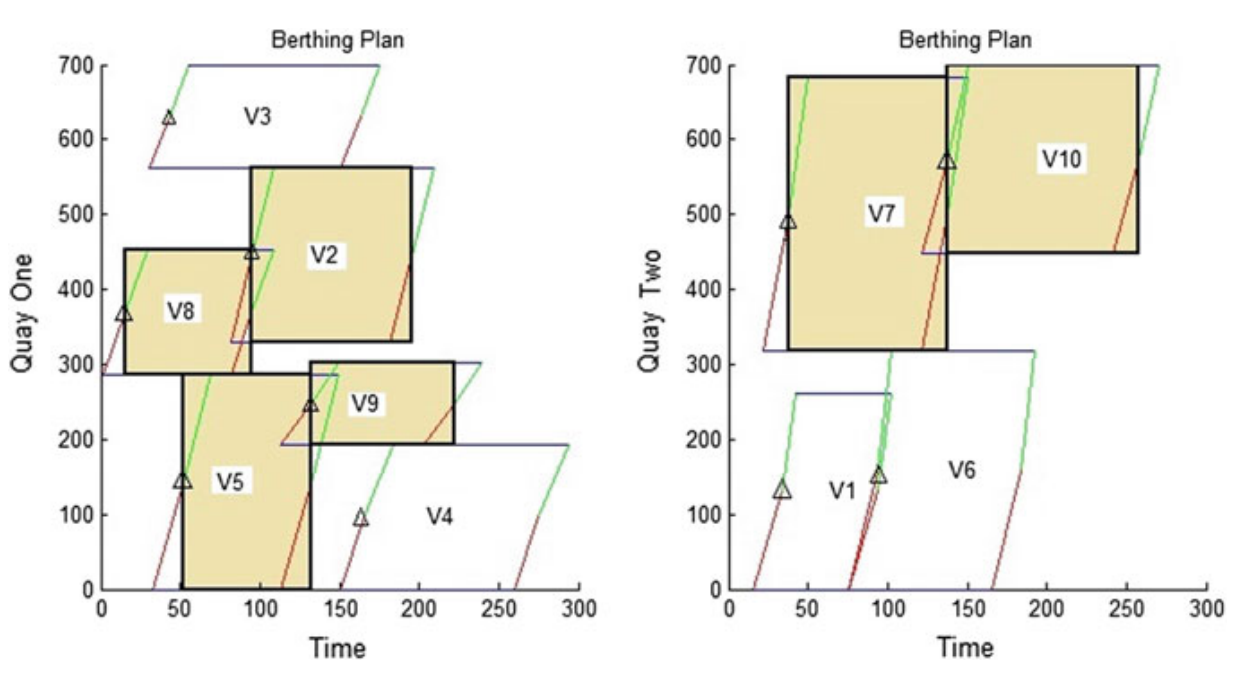
\includegraphics[width=.9\linewidth]{img/bap-example-fuzzy-solution.png}
\caption{\label{fig:bap-example-solution}Example solution of a fuzzy BAP model over multiple quays. The parallelograms represent the fuzzy solution visually by depicting the lower and upper bounds for the arrival and departure times with the vertial sloped lines. The yellow filled squares represent the average crisp solution.}
\end{figure}

\subsection{The Fuzzy PAP}
\label{sec:the-fuzzy-pap}
This section derives the Fuzzy PAP (FPAP). It is separated into three parts to construct each component individually:
objective function, queuing constraints, and charging constraints. Before deriving the FPAP, it is prudent to define the
set of fuzzy variables. Similarly to the Fuzzy BAP, the arrival times, \(\tilde{a}_i\), berthing time \(\tilde{u}_i\), and
detach time from the charger \(\tilde{d}_i\) are assumed to be imprecise. Thus, indirectly, the service time,
\(\tilde{s}_i\), the linearization constraint in \ref{eq:slack_gain}, \(\tilde{g}_{iq}\), and the initial charge for visit
\(i\), \(\tilde{\eta}_i\) will also become fuzzy values.

\subsubsection{Objective Function}
\label{sec:orgbdd914c}
Begin by rewriting the crisp objective function with the fuzzy linearization term as shown in \ref{eq:fuzzy-objective}.

\begin{equation}
\label{eq:fuzzy-objective}
\text{min } \sum_{i=1}^{n_I} \sum_{q=1}^{n_Q} \Big( w_{iq} m_q + \tilde{g}_{iq} \epsilon_{q} \Big)
\end{equation}

As shown in \ref{sec:fully-fuzzy-linear-programming}, the method of handling the fuzzy values in the objective function is to
simply apply a ranking function. Let \(\mathfrak{R}\) be defined as the First Index of Yager as shown in \ref{eq:first-index-yager}.
The resulting objective function is shown in \ref{eq:fuzzy-objective-yager}.

\begin{equation}
\label{eq:fuzzy-objective-yager}
\text{min } \sum_{i=1}^{n_I} \sum_{q=1}^{n_Q} \Big( w_{iq} m_q + \mathfrak{R}(g_{iq}) \epsilon_{q} \Big)
\end{equation}

\subsubsection{Queuing Constraints}
\label{sec:org453d9a4}
To derive the queuing constraints, the set of crisp constraints that are of interest are rewritten in terms of the fuzzy
variables that have been identified prior as shown in \ref{eq:fuzzy-packing-constrs}. \ref{subeq:fp_m_time} fuzzifies all the
temporal terms. \ref{subeq:fp_m_valid_pos} and \ref{subeq:fp_m_sigma} duplicate the constraints \(|\tilde{u}_i|\) times.
Using triangular fuzzy numbers, that would imply constraints for the lower, middle, and upper bounds of the temporal
impreciseness. Similarly, \ref{subeq:fp_m_detach}-\ref{subeq:fp_m_valid_depart} are equivalent to their crisp
counterparts, but with fuzzified terms. \ref{subeq:fp_binaryspace} simply updates the binary decision term.

\begin{multicols}{2}
\begin{subequations} \label{eq:fuzzy-packing-constrs}
\begin{equation}
    \tilde{u}_i - \tilde{u}_j - \tilde{s}_j - (\sigma_{ij} - 1)T \geq 0 \label{subeq:fp_m_time}         \\
\end{equation}
\begin{equation}
    \sigma_{ij} + \sigma_{ji} + \psi_{ij} + \psi_{ji} \geq 1                     \label{subeq:fp_m_valid_pos}    \\
\end{equation}
\begin{equation}
    \sigma_{ij} + \sigma_{ji} \leq 1                                       \label{subeq:fp_m_sigma}        \\
\end{equation}
\begin{equation}
    \tilde{s}_i + \tilde{u}_i = \tilde{d}_i                       \label{subeq:fp_m_detach}       \\
\end{equation}
\begin{equation}
    \tilde{a}_i \leq \tilde{u}_i \leq (T - \tilde{s}_i)                 \label{subeq:fp_m_valid_starts} \\
\end{equation}
\begin{equation}
    \tilde{d}_i \leq \tau_i                                             \label{subeq:fp_m_valid_depart} \\
\end{equation}
\begin{equation}
   \sigma_{ij}, \psi_{ij} \in \{0,1\}\;                                   \label{subeq:fp_binaryspace}        \\
\end{equation}
\end{subequations}
\end{multicols}

\subsubsection{Charging Constraints}
\label{sec:org9230bd2}
Similarly to the other derivations, the crisp constraints are rewritten with their equivalent fuzzy terms.
\ref{subeq:fp_init_charge}-\ref{subeq:fp_final_charge} are equivalent to their crisp counterpart with the added lower
and upper bounds for the battery charge for visit \(i\). Note that the discharge amount, \(\Delta_i\), is not fuzzy. It is
assumed that the bus traveled the same distance during the route, thus the same amount of discharge, but can be early,
on time, or late to the station. \ref{subeq:fp_gpgret}-\ref{subeq:fp_gwles} fuzzify the linearization terms in a similar
manner, but the crisp spatial term, \(w_{iq}\) is included. The inclusion of the crisp terms with the fuzzy values is
allowed because although the time may be allowed to fluctuate, the specified queue, discharge amounts, or initial/final
charges are the same for each element of the fuzzy temporal values. Thus, when the fuzzy constraints are converted into
crisp constraints, the constraint validity is maintained \cite{ghanbari-2019-fuzzy}.

\begin{multicols}{2}
\begin{subequations}                                                       \label{eq:fuzzy-dyn-constrs}
\begin{equation}
    \tilde{\eta}_{\Gamma^0_i} = \alpha \kappa_{\Gamma^0_i}                                        \label{subeq:fp_init_charge}    \\
\end{equation}
\begin{equation}
    \tilde{\eta}_i + \sum_{q=1}^{n_Q} \tilde{g}_{iq} r_q - \Delta_i = \tilde{\eta}_{\gamma_i} \label{subeq:fp_next_charge}    \\
\end{equation}
\begin{equation}
    \tilde{\eta}_i + \sum_{q=1}^{n_Q} \tilde{g}_{iq} r_q - \Delta_i \geq \nu \kappa_{\Gamma_i}       \label{subeq:fp_min_charge}     \\
\end{equation}
\begin{equation}
    \tilde{\eta}_i + \sum_{q=1}^{n_Q} \tilde{g}_{iq} r_q \leq \kappa_{\Gamma_i}               \label{subeq:fp_max_charge}     \\
\end{equation}
\begin{equation}
    \tilde{\eta}_{\Gamma^f_i} \geq \beta \kappa_{\Gamma^f_i}                                        \label{subeq:fp_final_charge}   \\
\end{equation}
\begin{equation}
    \tilde{s}_i - (1 - w_{iq})M \leq \tilde{g}_{iq}                           \label{subeq:fp_gpgret}         \\
\end{equation}
\begin{equation}
    \tilde{s}_i \geq \tilde{g}_{iq}                                           \label{subeq:fp_gples}          \\
\end{equation}
\begin{equation}
    Mw_{iq} \geq \tilde{g}_{iq}                                               \label{subeq:fp_gwgret}         \\
\end{equation}
\begin{equation}
    0 \leq \tilde{g}_{iq}                                                     \label{subeq:fp_gwles}          \\
\end{equation}
\end{subequations}
\end{multicols}

The penalty function, introduced under \ref{sec:obj-math-model-robust}, logically fits under the objective to provide a more
robust solution as its intent is to widen the solution space; however, the mathematics to develop the penalty method is
introduced in the objective function in the same way as the consumption and demand costs. The actions taken to develop
the penalty function will therefore be presented in tandem with the consumption and demand costs next.

\section{Minimize the monetary cost of charging the BEBs}
\label{sec:minimize-monetary-cost}
This section discusses the actions associated with the objective to minimize the monetary cost of charging the BEBs. To
accomplish the task, an objective function is incrementally developed to introduce the components of the assignment and
power costs. The assignment cost encodes the minimization of the chargers and encouraged use of slow chargers, as
discussed in \ref{sec:math-model-pap}. The assignment cost also introduces the penalty function, for the objective in
\ref{sec:obj-math-model-robust}, in an attempt to broaden the solution space of the MILP. The power cost component
encompasses the consumption and demand costs which will be derived. The method of more aggressively reducing demand cost
for peak hours is also introduced with the power cost component.

\subsection{Objective Function}
\label{sec:objective-function}
The objective function is used to compare the fitness of different candidate solutions against one another. This
objective function takes in input and decision variables to calculate some value of measure. The calculated objective
function value can either be maximized or minimized. The desired option is dependent on the problem to be solved as well
as the formulation of said objective function. Let \(J\) represent the objective function. The objective function for this
problem has four main considerations: charger assignment, consumption cost, demand cost, and sufficient charge.

Suppose the objective function is of the form \(\text{min } J = \AC + \PC\). \(\AC\) is the assignment cost, and \(\PC\) is
the power usage cost. The assignment cost represents the costs of assigning a bus to a particular queue as well as the
chosen charging period, \([u_i, d_i]\), as shown in \ref{eq:ac}. \(v_i \in \Qset\) is the charger index, \(u_i\) is the initial
charge time, \(d_i\) is the detach time for visit \(i\), \(\phi_i\) is a binary decision variable, \(m\) is the minimum charge
percentage allowed, \(\kappa_i\) is the battery capacity for visit \(i\), and \(\eta_i\) is the charge for \(b_i\) when it
arrives for visit \(i\).

\begin{equation}
\label{eq:ac}
\AC = \sum_{i=1}^I \Big(\epsilon_{v_i}r_q + \frac{1}{2} C \phi_i (\eta_i - m \kappa_i)^{2}\Big)
\end{equation}

The first term in the summation represents the calculation of the cost for assigning a bus to queue \(q\). If \(\epsilon_{vi}\) is
taken to be \(\epsilon_{v_i} = 1000v_i\), the objective function encourages the model to minimize the total amount of chargers.
Taking this a step further, if the model represents the first \(n_{Q_s}\) indices to be slow chargers and the next
\(n_{Q_f}\) indices to be fast chargers, where \(n_{Q_s} < n_{Q_f} \in \mathcal{Z}\) and \(n_{Q_s} + n_{Q_f} = Q\), the model will also encourage the use of slow
chargers over fast. The second term is the penalty function that is either enabled or disabled by \(\phi_i\)
\cite{luenberger-2008-penal-barrier-method}. \(\phi_i\) is enabled when the initial charge, \(\eta_i\), is less than the allowed
minimum charge, \(m\kappa_{b_i}\). This is further discussed in \ref{sec:constraints}. Note that the variables \(\phi_i\) and \(\eta_i\) are
both decision variables that are being multiplied together. This is called a bilinear term. Using a traditional MILP
solver, this would require linearization \cite{rodriguez-2013-compar-asses}; however, because SA handles nonlinearities
easily these bilinear terms will be ignored \cite{radosavljevic-2018-metah-optim}.

The demand cost quantifies the amount of power being used over a given period and adjusts the cost accordingly. The
consumption cost calculates the total amount of power being consumed by the chargers. The consumption cost is merely the
summation of all the energy being used over all the active periods for each charger in the time horizon as written in
\ref{eq:consumption-cost}. \(r_{v_i}\) is the charge rate for the active charger \(v_i\) and is multiplied by the time that the
charger will be utilized, \(s_i\).

\begin{equation}
\label{eq:consumption-cost}
  \sum_{i=1}^I r_{v_i}s_i
\end{equation}

The demand cost is calculated based on 15 minute increments (0.25 hours). This cost is also referred to as the peak 15. The
average power used over an arbitrary 15-minute interval is represented by \ref{eq:p15}.

\begin{equation}
\label{eq:p15}
p_{15}(t) = 0.25 \int_{t-0.25}^{t} p(\tau) d\tau
\end{equation}

Worst case must be assumed to always ensure enough power is supplied; therefore, the maximum value found is retained as
represented in \ref{eq:pmax}.

\begin{equation}
\label{eq:pmax}
p_{max}(t) = \text{max}_{\tau \in [0,t]}p_{15}(\tau)
\end{equation}

A fixed minimum threshold, \(p_{fix}\), is introduced as a base power rate to be charged at. Let this fixed threshold be
defined as \(p_{fix}\). In a similar manner as \(p_{max}\), the maximum value is retained. Furthermore, let \(s_r\) define the
demand rate which has the units of \(\frac{\$}{kW}\).

\begin{equation}
\label{eq:pdem}
p_d(t) = \text{max}(p_{fix},p_{max}(t))s_r
\end{equation}

\ref{eq:pdem}, again, retains the largest \(p_{dem}\) value with a starting fixed value of \(p_{fix}\). To write the total power
demand at any discrete time, consider \ref{eq:discrete-power}. Let \(\omega_h \in \omega\) be the discrete power demand at time step \(h\)
where \(h \in \{ 1, 2, ..., H \} \subset \mathcal{Z}\) and \(H = \frac{T}{0.25}\). For conciseness of notation we will abuse \(t_h\) to denote
the time in discrete form (as opposed to \(t\) being continuous), let \(dt_h = t_h - t_{h-1}\), and \(\Hset = \{ 1, 2, ..., H
\}\). Let \(\iota_h\) be a binary decision variable that is enabled if charger \(v_i \in \Qset\) is enabled in the time frame
\(dt_h\). Let the power usage of charger \(v_i\) be denoted as \(r_{v_i}\).

\begin{equation}
\label{eq:discrete-power}
  \omega_h = \sum_i^I \iota_h \cdot r_{v_i}
\end{equation}

The average power can be rewritten as \(p_{15}^h = \omega_h\), \(p_d\) can be rewritten as \(p_d^h = \text{max}_{h \in \Hset}
(p_{15}^{h})\), there the \(h\) repesents the \(h^{\text{th}}\) step. Finally, \(p_d^f\) can be written as \ref{eq:pd-dis}.

\begin{equation}
\label{eq:pd-dis}
  p_d^h = \text{max}_{h \in \Hset}(p_{fix}, p_{max}^h)s_d
\end{equation}

To write the power cost, \ref{eq:consumption-cost} and \ref{eq:pd-dis} are added together to create \ref{eq:pc}.

\begin{equation}
\label{eq:pc}
\PC = p^h_d + \sum_{i=1}^I \Big( r_{v_i}s_i \Big)
\end{equation}

\subsection{Constraints}
\label{sec:constraints}
Now that a method of calculating the fitness of a schedule has been established, a method for determining the
feasibility of a schedule must be defined. Feasible schedules require that the schedule maintain a certain list of
properties. These properties are enforced by a set of constraints derived from the MILP PAP. The constraints must ensure
no overlap temporally or spatially, receives enough charge to complete route after each visit \(i\), bus visit \(i\) cannot
be over-charged, and departs on time. The aforementioned constraints are shown in \ref{eq:constraints}.

\begin{multicols}{2}
\begin{subequations}
  \begin{equation}
      \label{seq:c0}
      u_i - d_j - (\sigma_{ij} - 1)T \ge 0
  \end{equation}
  \begin{equation}
      \label{seq:c1}
      v_i - v_j - 1 - (\psi_{ij} - 1)Q \ge 0
  \end{equation}
  \begin{equation}
      \label{seq:c2}
      \sigma_{ij} + \sigma_{ji} \le 1
  \end{equation}
  \begin{equation}
     \label{seq:c3}
      \psi_{ij} + \psi_{ji} \le 1
  \end{equation}
  \begin{equation}
      \label{seq:c4}
      \sigma_{ij} + \sigma_{ji} + \psi_{ij} + \psi_{ji} \ge 1
  \end{equation}
  \begin{equation}
      \label{seq:c5}
      \Delta_i = \delta_i \rho_i
  \end{equation}
  \begin{equation}
      \label{seq:c6}
      s_i = d_i - u_i
  \end{equation}
  \begin{equation}
      \label{seq:c7}
       \eta_{\xi_i} = \eta_{i} + r_{v_i}s_i - \Delta_i
  \end{equation}
  \begin{equation}
      \label{seq:c8}
       \eta_{i} + r_{v_i}s_i - \Delta_i \ge \nu \kappa_{\Xi_i}
  \end{equation}
  \begin{equation}
      \label{seq:c9}
      \kappa_{\Xi_i} \geq \eta_{i} + r_{v_i}s_i
  \end{equation}
  \begin{equation}
      \label{seq:c10}
      \eta_{i} - m\kappa_{b_i} \le T (1 - \phi_{i})
  \end{equation}
  \begin{equation}
      \label{seq:c11}
      m_{k_i} - \eta_{i} > T \phi_{i}
  \end{equation}
  \begin{equation}
      \label{seq:c12}
      a_i \leq u_i \leq d_i \le e_i \le T
  \end{equation}
  \begin{equation}
      \label{seq:c13}
      u_i - dt_h \le T\theta_h
  \end{equation}
  \begin{equation}
      \label{seq:c14}
      dt_h - u_i \le T(1 - \theta_h)
  \end{equation}
  \begin{equation}
      \label{seq:c15}
      dt_h - d_i \le T\mu_h
  \end{equation}
  \begin{equation}
      \label{seq:c16}
      d_i - dt_h \le T(1 - \mu_h)
  \end{equation}
  \begin{equation}
      \label{seq:c17}
      \iota_h = \mu_h \theta_h
  \end{equation}
\end{subequations}
\label{eq:constraints}
\end{multicols}

Constraints \ref{seq:c0}-\ref{seq:c4} are the ``queuing constraints''. They are preventing overlap in both spatially and
temporally as shown in \ref{fig:spacial-and-temporal-constr}. The y-axis represents the possible queues for a bus visit to be
placed into, and the x-axis represents the time that can be reserved for each visit. The shaded rectangles represent
time that has been scheduled, and the queue allocated for each bus visit. The set of constraints \ref{seq:c0} -
\ref{seq:c4} aim to ensure that these shaded rectangles never overlap.

\begin{figure}[ht!]
  \centering
  \scalebox{0.5}{
  \centerline{
    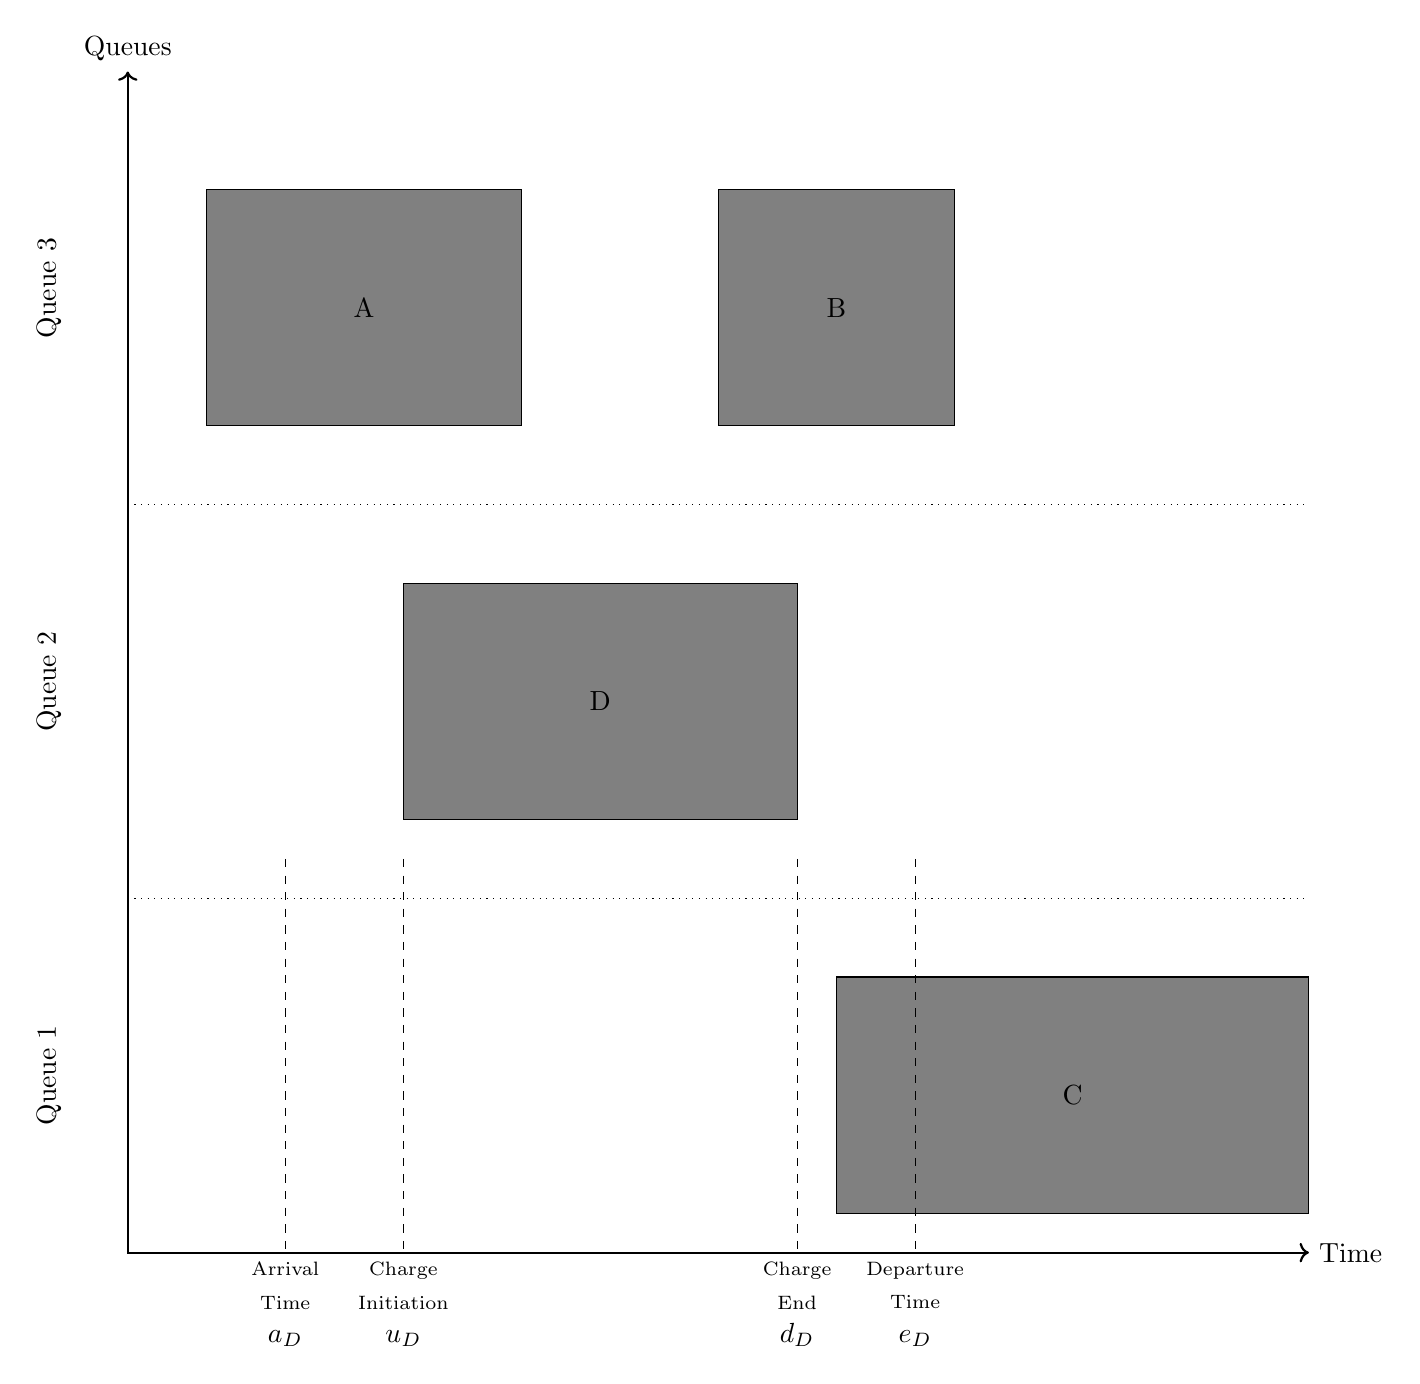
\begin{tikzpicture}
      % Variables
      \def \arrx   {2.0}
      \def \initx  {3.5}
      \def \endx   {8.5}
      \def \depx   {10.0}
      \def \yshift {5}

      % Axis
      \draw [thick,<->] (0,15) node[above]{Queues} -- (0,0) -- (15,0) node[right]{Time};

      % Rectangles
      \node[rectangle, draw, fill=gray, minimum width=4cm, minimum height = 3cm] at (3,12) {A};
      \node[rectangle, draw, fill=gray, minimum width=3cm, minimum height = 3cm] at (9,12) {B};
      \node[rectangle, draw, fill=gray, minimum width=5cm, minimum height = 3cm] at (6,7) {D};
      \node[rectangle, draw, fill=gray, minimum width=6cm, minimum height = 3cm] at (12,2) {C};

      % X-axis labels
      \node [below,align=center] at (\arrx,0) {\scriptsize Arrival     \\ \scriptsize Time \\ $a_D$};
      \node [below, align=center] at (\initx,0) {\scriptsize Charge    \\ \scriptsize Initiation  \\ $u_D$};
      \node [below, align=center] at (\endx,0) {\scriptsize Charge     \\ \scriptsize End \\ $d_D$};
      \node [below, align=center] at (\depx,0) {\scriptsize Departure  \\ \scriptsize Time \\ $e_D$};

      % Y-axis labels
      \node[rotate=90] at (-1, 2.25) {Queue 1};
      \node[rotate=90] at (-1, 7.25) {Queue 2};
      \node[rotate=90] at (-1, 12.25) {Queue 3};

      % Vertical lines
      \draw[dashed] (\arrx,\yshift)--(\arrx,0);
      \draw[dashed] (\initx,\yshift)--(\initx,0);
      \draw[dashed] (\endx,\yshift)--(\endx,0);
      \draw[dashed] (\depx,\yshift)--(\depx,0);

      % Horizontal lines
      \draw[dotted] (0, 4.5) -- (15, 4.5);
      \draw[dotted] (0, 9.5) -- (15, 9.5);

    \end{tikzpicture}
  }}
  \caption{Visualization of the temporal and spatial aspect of the aspect of the schedule. The grey rectangle labeled $D$ represents the time that the charger in queue 2 is active. $a_D$ represents the arrival time for bus $D$. The diagram indicates that $D$ arrives prior to the inital charge time, $u_D$. $d_D$ is the detatch time for bus $D$, which is before the departure time $e_D$. Physically, that represents bus $D$ being idle between $a_D$ and $u_D$ while its waiting to be charged, charging between $u_D$ and $d_D$, and idle again between $d_D$ and $e_D$ waiting to depart on the next route.}
  \label{fig:spacial-and-temporal-constr}
\end{figure}

Constraint \ref{seq:c4} states that the starting service time for bus \(j\), \(u_j\), must be greater than the starting time
of bus \(i\), \(u_i\), plus its service time, \(s_i\). The last term utilizes big-M notation to activate or deactivate the
constraint. A value of \(\sigma_{ij} = 1\) will activate the constraint to ensure that bus \(i\) is complete before bus \(j\) is
allowed to begin being serviced. If \(\sigma_{ij} = 0\), then the constraint is of the form \(T + u_j + s_j > u_i\) rendering the
constraint ``inactive'' because \(u_i\) cannot be larger than \(d_i\). This effectively allows the charging windows of the
vehicle to overlap.

Similarly, \(\phi_{ij}\) determines whether the vehicles will be charging in the same queue. If \(\phi_{ij} = 1\) then
\eqref{seq:c1} is rendered active and vehicle \(i\) and \(j\) must be charging in different queues. If \(\phi_{ij} = 0\) then the
constraint is deactivated and the vehicle queue assignments may be the same.

\ref{seq:c5} calculates the discharge for the route after visit \(i\). \ref{seq:c6} describes the service time of the bus.
\ref{seq:c7} calculates the initial charge for the next visit for bus \(b_i\). \ref{seq:c7} ensures that the bus is not
being over-charged. \ref{seq:c9} and \ref{seq:c10} are used to enable and disable the penalty method in \ref{eq:ac}. This is
done by checking if the initial charge for visit \(i\) is greater than or equal to the minimum allowed charge.
\ref{seq:c10} ensures the continuity of the times (i.e. the arrival time is less than the initial charge which is less
than the detach time which is less than the time the bus exits the station and all must be less than the time horizon).

The last set of constraints \ref{seq:c13} - \ref{seq:c17} set the rules for the decision variable \(\iota_h\). \ref{seq:c13}
and \ref{seq:c14} ensure that the initial charge time for visit \(i\), \(u_i\), is greater than the discrete time, \(0.25 \cdot
h\), being checked. Similarly, \ref{seq:c15} and \ref{seq:c16} ensure that the final charge time, \(d_i\), is less than the
next discrete time step, \(dt_h\). The final constraint \ref{seq:c17} is the discrete representation of whether charger
\(v_i \in \Qset\) is active.

\section{Method And Validation}
\label{sec:org2df36fe}
The proposed work is to be modeled and simulated using a SA approach written in the Rust programming language. Rust has
been chosen for its reliability with its ownership model, performance that is comparable to C/C++, and its Python-like
packaging system. SA was chosen as for its simplicity in implementation, and is one of the best known metaheuristic
methods for ``addressing difficult black global optimization problems'' \cite{delahaye-2019-simul}. Note that the SA-PAP
implementation has begun. At the moment the main development that has been completed is: project structure/design,
implementation of the skeletal framework, code for importing route data, and some work has been done on the generating
functions. As previously stated, the MILP-PAP has been implemented and tested. Thus, the MILP-PAP shall be used as a
baseline measure to compare the results of the proposed work. An introduction to Simulated Annealing as well as the
proposed method of implementation will subsequently be outlined and discussed.

\subsection{Simulated Annealing}
\label{sec:simulated-annealing}
SA is an exploitation oriented, single-solution based (as compared to population based) metaheuristic approach in which
its main advantage is its simplicity both theoretically and in its implementation as well its inherit ability to
overcome nonlinearities \cite{gendreau-2018-handb-metah,radosavljevic-2018-metah-optim}. This model is named after its
analogized process where a crystalline solid is heated then allowed to cool very slowly until it achieves its most
regular possible crystal lattice configuration \cite{henderson-1989-theor-pract}. There are five key components to SA:
initial temperature, cooling schedule (temperature function), generation mechanism, acceptance criteria, local search
iteration count (temperature change counter) \cite{keller-2019-multi-objec}.

\subsubsection{Cooling Equation (Experimental)}
\label{cooling-equation-experimental}
The initial temperature and cooling schedule are used to regulate the speed at which the solution attempts to converge
to the best known solution. When the temperature is high, SA encourages exploration. As it cools down (in accordance to
the cooling schedule), it begins to encourage local exploitation of the solution
\cite{rutenbar-1989-simul-anneal-algor,henderson-1989-theor-pract}]. There are three basic types of cooling equations
as shown in \ref{fig:cool} \cite{keller-2019-multi-objec}. The different types merely dictate the rate at which the algorithm
progressively disallows exploration. A linear cooling schedule is defined by \ref{eq:cool0}.

\begin{equation}
\label{eq:cool0}
\Tau[n] = \Tau[n-1] - \Delta_0
\end{equation}

with \(\Tau[0] = \Tau_0\) and \(\Delta_0 = 1/2\; C^\circ\) in \ref{fig:cool}. A geometric cooling schedule is mostly used in practice
\cite{keller-2019-multi-objec}. It is defined by \ref{eq:cool1}.

\begin{equation}
\label{eq:cool1}
\Tau[n] = \alpha \Tau[n-1]
\end{equation}

where \(\alpha = 0.995\) in \ref{fig:cool}. An Exponential cooling schedule is defined by the difference equation is defined as
\ref{eq:cool2}.

\begin{equation}
\label{eq:cool2}
\Tau[n] = e^{\beta}\Tau[n-1]
\end{equation}

where \(\beta = 0.01\) in \ref{fig:cool}. The initial temperature, \(T_0\), in the case of \ref{fig:cool}, is set to \(500^\circ\; C\) and
each schedule's final temperature is \(1\; C^\circ\).

\begin{figure}[htbp]
\centering
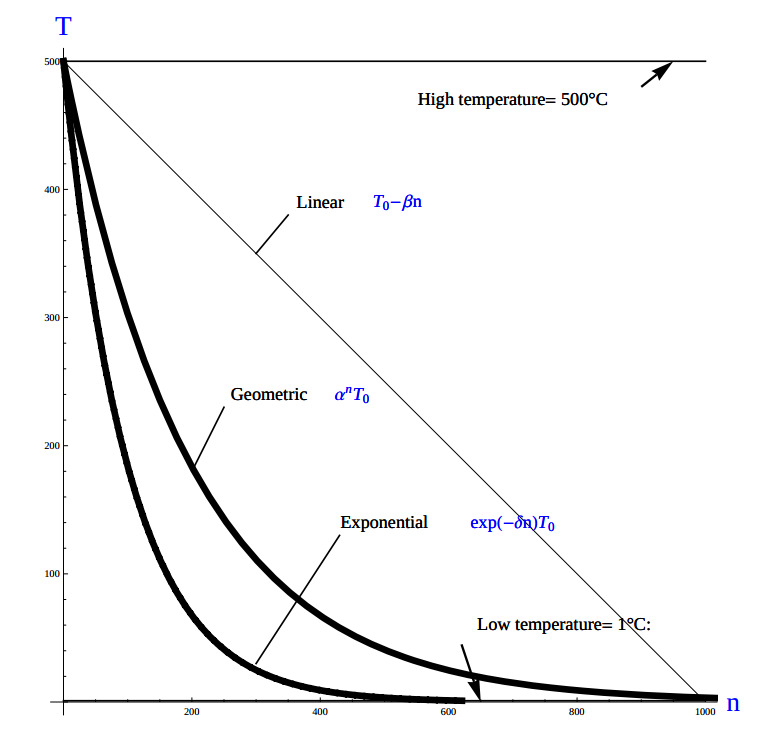
\includegraphics[width=0.5\textwidth]{img/cool-func.jpg}
\caption{\label{fig:cool}Cooling equations}
\end{figure}

\subsubsection{Acceptance Criteria}
\label{sec:acceptance}
Acceptance criteria describes the method to accept or reject a given candidate solution. In SA, if a new candidate
solution is more fit than the currently stored solution it is always accepted as the new solution. However, within SA,
worse candidate solutions may be accepted as the new solution. The probability of accepting the candidate solution is
described by the function \(\exp(-\frac{J(x) - J(x')}{\Tau})\) where \(J(\cdot)\) is the objective functions described in
\ref{sec:objective-function}. The probability of acceptance is a function of the cooling equation just described and
difference of the current solution and a new candidate solution. Let \(\Delta E \equiv J(x) - J(x')\) where \(x\) is the current
solution and \(x'\) is the new candidate solution. The probability of acceptance of \(x'\) is defined by \ref{eq:candaccept}
\cite{keller-2019-multi-objec}.

\begin{equation}
\label{eq:candaccept}
f(x,x',T) =
\begin{cases}
  1                 & \Delta E > 0 \\
  e^{- \frac{\Delta E}{T}} & \text{otherwise}
\end{cases}
\end{equation}

\subsubsection{Generation Mechanisms}
\label{sec:generation-mechanisms}
Generation mechanisms in SA are used to generate random solutions to propose to the optimizer, these are known as
candidate solutions. In the case of the problem statement made in \ref{sec:problem-description}, five generation mechanism
shall be used: new visit, slide visit, new charger, remove, new window. The purpose of each of these generators is to
assign new visits to a charger, adjust a bus visits initial and final charge time within the same time frame/queue,
remove a bus from a charger, and place a bus visit into a new time slot/queue. Each generator will be discussed in more
detail in \ref{sec:generators}.

These generator mechanisms will in turn be utilized by two wrapper functions. The schedule generation is to used create
candidate solutions for SA to compare with other solutions, and the perturb schedule generator is used to take a
candidate solution and alter it slightly in an attempt to fall into a global/local minimum.

\paragraph{Generator Input/Output}
\label{sec:generator-input-output}
This section discusses in detail the expected inputs and output of each generator. It is important to discuss these
parameters in order to have an understanding of the generating algorithms derived. The input consists of the bus visit
index of interest, information about the current state of arrivals, \(\I\), and the current state of the chargers'
availability, \(\C\). The output of each generator affects the tuple of decision variables \((v_i, u_i, d_i) \subset \I_i\).

\begin{enumerate}
\item Generator Input
\label{sec:org3709b2b}
Each generator has the tuple input of \(\Sol \equiv (i, \I, \C)\) where \(i\) is the visit index, \(\I_i\) is the tuple \(\visit\)
(\ref{sec:problem-description}), that describes the set of visits, and \(\C\) is the set that describes the availability for
all chargers \(q \in \Qset\). In other words, \(\C\) defines the set of times when the chargers are not being utilized or are
``inactive''.

To derive \(\C\), consider its inverse, \(\C'\), which is the set of ``active'' time periods for each charger, \(\C' = \bigcup
\{\C_q' : q \in \mathcal{Q}\}\) where \(\C_q' \subset \C'\) describes the active times for chagrer \(q\). Focusing on an individual charger,
consider \(\C_q'\) before a schedule has been imposed upon it, \(\C_q' \in \varnothing\). In other words, no buses have been
assigned to be charged over the time period of \([u_i, d_i]\). After the scheduling process is complete, \(\C_q'\) will have
a set of active periods of the form \(\C_q' \in \{[u_j, d_j]: j \in \Jsetq \}\) where \(\Jsetq \subset \mathcal{I}\). For \(\C_q'\) to be of
value, its compliment is to be found, \(\C_q\). Let \(j\text{th}\) inactive period shall be denoted as \(\C^j_q\).

To determine the inverse of \(\C_q'\), begin by noting \(\C_q' \bigcap \{[u_j, d_j] : j \in \Jsetq\} = \varnothing\), is said to be
disjoint \cite{halmos-1974-naive-set-theor}. The inverse of a disjoint set can be found by the De Morgan Law as shown
in \ref{eq:demorgan}. Using \ref{eq:demorgan}, the set of inactive periods can be written as \(\C_q \equiv \bigcup \{[u_j, d_j]': j \in \Jsetq\}\).
Let \(\Sol\) denote the tuple \(\Sol \equiv (i, \I, \C)\).

\begin{equation}
\label{eq:demorgan}
(A \cap B)' = A' \cup B'
\end{equation}

\item Generator Output
\label{sec:org8566c4b}
The output is a modified visit, noted as \(\I_i'\). In actuality only the decision variables are being altered which is a
subset of \(\I_i\). Let this subset be defined by \(x_i' \equiv (v_i, u_i, d_i) \subset \I_i\) which is the chosen queue, initial
charge time, and detach time from the generator, \((v_i, u_i, d_i)\). The nature of SA implies that the generators have a
sense of randomness. Because of that, some of the generators may have multiple choices for what \(x_i'\) may be. Let the
set of candidates for the output be defined as \(x_i' \in X_i'\). Furthermore, set the set of candidate visits be denoted as
\(\I_i' \in \I'\).
\end{enumerate}

\paragraph{Generators}
\label{sec:generators}
This section describes and outlines the algorithm pool for the different generator types that are utilized in the
wrapper functions. Note that to satisfy constraints, \(B\) extra idle queues that provide no power to the bus. Because of
this, the set of queues is fully defined as \(q \in \{1,..., Q, Q+1,..., Q+B\}\) where \(Q\) is the total amount of chargers
and \(b\) is the bus ID. The use case for this is for when a bus is not to be placed on a charger, it will be placed in
the queue, \(v_i \in \{Q+1,..., Q+B\}\), which will satisfy the constraints above while allowing the bus to be ``set aside''
while others charge.

\begin{enumerate}
\item New visit
\label{new-visit}
The new visit generator describes the process of moving bus \(b\) from the idle queue, \(v_i \in \{Q+1,..., Q+B\}\) to a valid
charging queue, \(v_i \in \{1,..., Q\}\). Lines 2-4 extracts the visit, \(i\), arrival time, \(a_i\), and departure time, \(e_i\).
Note that in subsequent algorithms these lines will be omitted for conciseness. Line 5 loops through the inactive time
periods that contain the time the bus is at the station, \([a_i, e_i]\). \(\U_{\cdot}\) indicates that an element is selected
randomly with a uniform distribution from the set \(\{\cdot\}\). Line 6 verifies that the inactive period selected is valid
and returns a random charging time, \([u_i, d_i]\), if it is. Line 7 returns the new visit.

\begin{algorithm}[H]
\caption{New visit algorithm} \label{alg:new-visit}
    \LinesNumbered
    \TitleOfAlgo{New Visit}
    \KwIn{($\Sol$)}
    \KwOut{$\I_i'$}

    \SetKwFunction{Union}{Union}
    \SetKwFunction{findFreeTime}{findFreeTime}

    \Begin
    {
        $i    \leftarrow \{i: i \in \Sol \}$ \tcc*{The index of the visit $i$}
        $a_i  \leftarrow \{ a_i \in \I_i : \I_i \in \I \subset \Sol \}$ \tcc*{Get the arrival time for visit $i$}
        $e_i  \leftarrow \{ e_i \in \I_i : \I_i \in \I \subset \Sol \}$ \tcc*{Get the departure time for visit $i$}

        \tcc{Randomly select a free time, $j$, from any charger $q \in \Qset$ that is within the time frame $[a_i e_i]$}
        \While {$C_q^j \in \{[a_i, e_i]\} \subset \U_{\C}$}
        {
            \If(\tcc*[f]{If there is time available in $C_q^j$}){$x_i' \leftarrow$ \findFreeTime{$C_q^j, (a_i, e_i)$} $\not\in \varnothing$}
            {
                \Return{$\I_i' \leftarrow x_i'$} \tcc*[f]{Return visit}
            }
        }
    }
\end{algorithm}

The function \texttt{findFreeTime} in \ref{alg:new-visit} is defined in \ref{alg:find-free-time}. \(L\) and \(U\) are the lower
and upper bound of the time between scheduled times. The possible use cases are depicted in \ref{fig:find-free}. In each case
depicted by \ref{fig:find-free}, the red line shows the arrival and departure time for an arbitrary bus visit, \(i\). The blue
lines indicate reigons in which charger \(q\) is active. \(C \in \C_q \subset \C\) represents one of the regions between the blue
lines, \([L, U]\) which stand for the lower and upper portions of the regions, respectively. The output of
\ref{alg:find-free-time}. That is, the only scheduling constraint is that the arrival time is before charger \(q\) is
available to charge the bus. Therefore, the bus must wait intil \(L\) before changer \(q\) may charge it. Furthermore, the
range that \(u_i\) must be selected from is \([L,e]\).

\begin{figure}
\centering
\begin{subfigure}{\textwidth}
    \centering
    \caption{Valid position: $a \leq u \leq d \leq e$}
    \label{subfig:sandwich}
    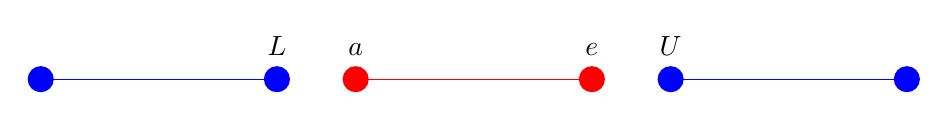
\begin{tikzpicture}[scale=2]
        \coordinate (A) at (0,0);
        \coordinate (B) at (1.5,0);
        \coordinate (C) at (2.0,0);
        \coordinate (D) at (3.5,0);
        \coordinate (E) at (4.0,0);
        \coordinate (F) at (5.5,0);

        \draw[blue] (A) -- (B);
        \draw[red]  (C) -- (D);
        \draw[blue] (E) -- (F);

        \node[circle,fill=blue,radius=0.15]                     at (A) {};
        \node[circle,fill=blue,radius=0.15,label=above : $L$]   at (B) {};
        \node[circle,fill=red,radius=0.15,label=above  : $a$] at (C) {};
        \node[circle,fill=red,radius=0.15,label=above  : $e$] at (D) {};
        \node[circle,fill=blue,radius=0.15,label=above : $U$]   at (E) {};
        \node[circle,fill=blue,radius=0.15]                     at (F) {};
    \end{tikzpicture}
\end{subfigure}

\par\bigskip

\begin{subfigure}{\textwidth}
    \centering
    \caption{Valid position: $L \leq u \leq d \leq e$}
    \label{subfig:all}
    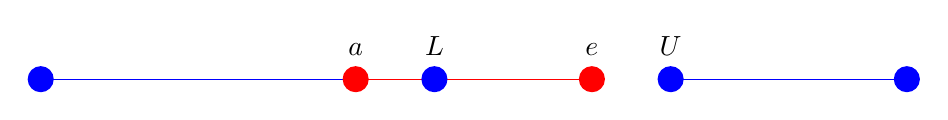
\begin{tikzpicture}[scale=2]
        \coordinate (A) at (0,0);
        \coordinate (B) at (2.5,0);
        \coordinate (C) at (2.0,0);
        \coordinate (D) at (3.5,0);
        \coordinate (E) at (4.0,0);
        \coordinate (F) at (5.5,0);

        \draw[blue] (A) -- (B);
        \draw[red]  (C) -- (D);
        \draw[blue] (E) -- (F);

        \node[circle,fill=blue,radius=0.15]                     at (A) {};
        \node[circle,fill=blue,radius=0.15,label=above : $L$]   at (B) {};
        \node[circle,fill=red,radius=0.15,label=above  : $a$] at (C) {};
        \node[circle,fill=red,radius=0.15,label=above  : $e$] at (D) {};
        \node[circle,fill=blue,radius=0.15,label=above : $U$]   at (E) {};
        \node[circle,fill=blue,radius=0.15]                     at (F) {};
    \end{tikzpicture}
\end{subfigure}

\par\bigskip

\begin{subfigure}{\textwidth}
    \centering
    \caption{Valid position: $a \leq u \le d \leq U$}
    \label{subfig:egu}
    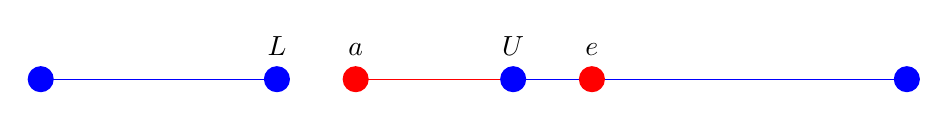
\begin{tikzpicture}[scale=2]
        \coordinate (A) at (0,0);
        \coordinate (B) at (1.5,0);
        \coordinate (C) at (2.0,0);
        \coordinate (D) at (3.5,0);
        \coordinate (E) at (3.0,0);
        \coordinate (F) at (5.5,0);

        \draw[blue] (A) -- (B);
        \draw[red]  (C) -- (D);
        \draw[blue] (E) -- (F);

        \node[circle,fill=blue,radius=0.15]                     at (A) {};
        \node[circle,fill=blue,radius=0.15,label=above : $L$]   at (B) {};
        \node[circle,fill=red,radius=0.15,label=above  : $a$] at (C) {};
        \node[circle,fill=red,radius=0.15,label=above  : $e$] at (D) {};
        \node[circle,fill=blue,radius=0.15,label=above : $U$]   at (E) {};
        \node[circle,fill=blue,radius=0.15]                     at (F) {};
    \end{tikzpicture}
\end{subfigure}

\par\bigskip

\begin{subfigure}{\textwidth}
    \centering
    \caption{Valid position: $L \le u \leq d \leq U$}
    \label{subfig:invertsandwhich}
    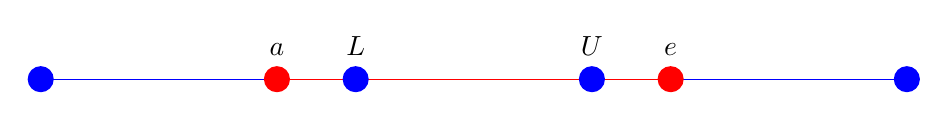
\begin{tikzpicture}[scale=2]
        \coordinate (A) at (0,0);
        \coordinate (B) at (1.5,0);
        \coordinate (C) at (2.0,0);
        \coordinate (D) at (3.5,0);
        \coordinate (E) at (4.0,0);
        \coordinate (F) at (5.5,0);

        \draw[blue] (A) -- (C);
        \draw[blue] (D) -- (F);
        \draw[red]  (B) -- (E);

        \node[circle,fill=blue,radius=0.15]                    at (A) {};
        \node[circle,fill=red,radius=0.15,label=above : $a$]   at (B) {};
        \node[circle,fill=blue,radius=0.15,label=above  : $L$] at (C) {};
        \node[circle,fill=blue,radius=0.15,label=above  : $U$] at (D) {};
        \node[circle,fill=red,radius=0.15,label=above : $e$]   at (E) {};
        \node[circle,fill=blue,radius=0.15]                    at (F) {};
    \end{tikzpicture}
\end{subfigure}

\par\bigskip

\begin{subfigure}{\textwidth}
    \centering
    \caption{Invalid position upper bound}
    \label{subfig:invalid-upper}
    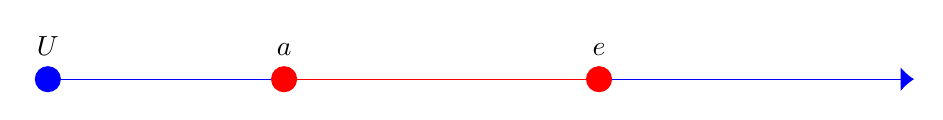
\begin{tikzpicture}[scale=2]
        \coordinate (A) at (0.0,0);
        \coordinate (B) at (5.5,0);
        \coordinate (C) at (1.5,0);
        \coordinate (D) at (3.5,0);

        \draw[-{Latex[width=3mm]},blue]  (A) -- (B);
        \draw[red]  (C) -- (D);

        \node[circle,fill=blue,radius=0.15,label=above : $U$] at (A) {};
        \node[circle,fill=red,radius=0.15,label=above  : $a$] at (C) {};
        \node[circle,fill=red,radius=0.15,label=above  : $e$] at (D) {};
    \end{tikzpicture}
\end{subfigure}

\par\bigskip

\begin{subfigure}{\textwidth}
    \centering
    \caption{Invalid position lower bound}
    \label{subfig:invalid-lower}
    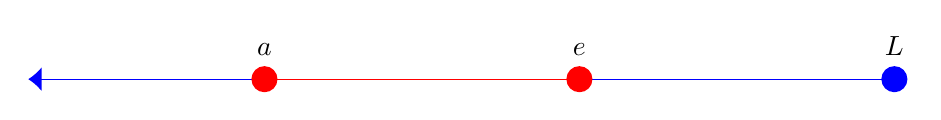
\begin{tikzpicture}[scale=2]
        \coordinate (A) at (0.0,0);
        \coordinate (B) at (5.5,0);
        \coordinate (C) at (1.5,0);
        \coordinate (D) at (3.5,0);

        \draw[-{Latex[width=3mm]},blue]  (B) -- (A);
        \draw[red]  (C) -- (D);

        \node[circle,fill=blue,radius=0.15,label=above : $L$] at (B) {};
        \node[circle,fill=red,radius=0.15,label=above  : $a$] at (C) {};
        \node[circle,fill=red,radius=0.15,label=above  : $e$] at (D) {};
    \end{tikzpicture}
\end{subfigure}

\caption{Outlines the different cases that requested time and charger allocated time can overlap}
\label{fig:find-free}
\end{figure}

\begin{algorithm}[H]
\caption{Find free time algorithm searches and returns the available time frames} \label{alg:find-free-time}
    \LinesNumbered
    \TitleOfAlgo{Find Free Time}
    \KwIn{$(L,U,a,e)$}
    \KwOut{$(u,d)$}

    \Begin
    {
        \If(\tcc*[f]{If $L < a < e < U]$ (\autoref{subfig:sandwich})}){$L \leq a$ and $U \geq e$}
        {
                u $\leftarrow$ $\U_{[a,e]}$\;
                d $\leftarrow$ $\U_{[u,e]}$\;
        }
        \ElseIf(\tcc*[f]{Else if $a < L < e < U$ (\autoref{subfig:all})}){$L > a$ and $U \geq e$}
        {
                u $\leftarrow$ $\U_{[L,e]}$\;
                d $\leftarrow$ $\U_{[u,e]}$\;
        }
        \ElseIf(\tcc*[f]{Else if $L < a < U < e$ (\autoref{subfig:egu})}){$L \leq a$ and $U < e$}
        {
                u $\leftarrow$ $\U_{[a,U]}$\;
                d $\leftarrow$ $\U_{[u,U]}$\;
        }
        \ElseIf(\tcc*[f]{Else if $a \leq u \leq d \leq L$ or $U \leq a \leq d \leq e$ (\autoref{subfig:invertsandwhich})}){$L > a$ and $U < e$}
        {
                u $\leftarrow$ $\U_{[a,L], [U,e]}$\;
                d $\leftarrow$ $\U_{[u,L], [u,e]}$\;
        }
        \Else(\tcc*[f]{Otherwise the bus cannot be scheduled in this time frame (\autoref{subfig:invalid-lower}, \autoref{subfig:invalid-upper})})
        {
                u $\leftarrow$ $\varnothing$\;
                d $\leftarrow$ $\varnothing$\;
        }

        \Return{(u,d)}
    }
\end{algorithm}

\item Slide visit
\label{slide-visit}
Slide visit (\ref{alg:slide-visit}) is used for buses that have already been scheduled. Because of the constraint
\ref{seq:c10} there may be some room to move \(u_i\) and \(d_i\) within the window \([a_i, e_i]\). Two new values, \(u_i\) and
\(d_i\) are selected with a uniform distribution to satisfy the constraint \(a_i \leq u_i \leq d_i \leq e_i\). Line 2 randomly loops
through the other inactive time frames from charger \(v_i\) that is within the time that the bus is at the station, \([a_i,
e_i]\). Line 3 verifies the time frame previously selected and returns a new charging time. Line 4 returns the new visit.

\begin{algorithm}[H]
\caption{Slide Visit Algorithm} \label{alg:slide-visit}
    \LinesNumbered
    \TitleOfAlgo{Slide Visit}
    \KwIn{$\Sol$}
    \KwOut{$\I_i'$}

    \Begin
    {
        \tcc{Randomly select an inactive time frame, $j$, from charger $v_i$ that is within the time frame $[a_i, e_i]$}
        \While {$C_q^j \in \{[a_i, e_i]\} \subset \U_{\C_{v_i}}$}
        {
            \If(\tcc*[f]{If there is time available in $C_q^j$}){$x_i' \leftarrow$ \findFreeTime{$C_q^j$, ($a_i, e_i$)} $\not\in \varnothing$}
            {
                \Return{$\I_i \leftarrow x_i'$} \tcc*[f]{Return visit}
            }
        }
    }
\end{algorithm}

\item New charger
\label{new-charger}
The new charger generator takes a visit \(\I_i\) and changes the charger it is on while maintianing the same charge time,
\([u_i, d_i]\). Similar to \ref{alg:new-visit}, the new candidate, \(x_i'\), must be checked before being added to the set \(X_i'\).
Line 2 randomly loops through any time frame from any charger, \(C_q^j\), that is within the time frame that the bus is at
the station, \([a_i, e_i]\). Line 3 verifies the selection and line 4 returns the new visit.

\begin{algorithm}[H]
\caption{New Charger Algorithm} \label{alg:new-charger}
    \LinesNumbered
    \TitleOfAlgo{New Charger}
    \KwIn{$\Sol$}
    \KwOut{$\I_i'$}

    \Begin
    {
        \tcc{Randomly select an inactive time frame, $j$, from any charger $q \in \Qset$ that is within the time frame $[a_i, e_i]$}
        \While {$C_q^j \in \{[a_i, e_i] \} \subset \U_{\C}$}
        {
            \If (\tcc*[f]{If the charge time is within the region $[L,U]$}) {$L \leq u_i$ \And $U \geq d_i$}
            {
                \Return{$\I_i \leftarrow x_i'$} \tcc*[f]{Return visit}
            }
        }

    }
\end{algorithm}

\item Remove
\label{sec:remove}
The remove generator simply removes a bus from a charger queue and places it in its idle queue, \(v_i \in
\{Q,...,Q+B\}\).

\begin{algorithm}[H]
\caption{Remove algorithm} \label{alg:remove}
    \LinesNumbered
    \TitleOfAlgo{Remove}
    \KwIn{$\Sol$}
    \KwOut{$\I_i'$}

    \Begin
    {
       \Return{$\I_i' \leftarrow (Q+b,a_i,e_i)$}
    }
\end{algorithm}

\item New Window
\label{sec:new-visit}
New window is a combination of the remove and then new visit generators (\ref{sec:remove} and \ref{sec:new-visit}). By this it is
meant that current scheduled tuple \((v_i, u_i, d_i)\) is removed and added back in as if it were a new visit.

\begin{algorithm}[H]
\caption{New window algorithm}
    \LinesNumbered
    \TitleOfAlgo{New Window}
    \KwIn{$\Sol$}
    \KwOut{$\I_i'$}

    \Begin
    {
        \SetKwFunction{NewVisit}{NewVisit}
        \SetKwFunction{Remove}{Remove}

        $\I_i' \leftarrow$ \Remove{$v,u,d$}   \tcc*{Remove visit $i$ from its charger}
        $\Sol \leftarrow \I_i'$               \tcc*{Update the route information tuple}
        $\I_i' \leftarrow$ \NewVisit{$\Sol'$} \tcc*{Add visit $i$ back in randomly}

        \Return{$(v,u,d)$}
    }
\label{alg:new-window}
\end{algorithm}
\end{enumerate}

\paragraph{Generator Wrappers}
\label{generator-wrappers}
This section covers the algorithms utilized to select and execute different generation processes for the SA process. The
generator wrappers are the method immediately called by SA. Each wrapper utilizes the generators previously described
and returns either metadata about the bus routes or a new valid charger schedule.

\begin{enumerate}
\item Schedule Generation
\label{schedule-generation}
The objective of this generator is to generate a candidate solution to the given schedule. To generate a candidate
solution, the generator is given \(\I\), a bus is picked at random, \(b \in \Bset\), then a random visit is picked. The new
visit generator (\ref{alg:new-visit}) is then utilized. This process is repeated for each visit. This algorithm is
summarized in \ref{alg:schedule-generation}. Recall from \ref{sec:input-variables}, \(\Jset_B \subset \I\) is used to indicate the
set of visit indices for bus \(b\).

\begin{algorithm}[H]
\caption{Schedule generation algorithm} \label{alg:schedule-generation}
    \LinesNumbered
    \TitleOfAlgo{ScheduleGeneration}
    \KwIn{$\I$, $\C$}
    \KwOut{$\I'$, $\C'$}

    \SetKwFunction{Union}{Union}
    \SetKwFunction{NewVisit}{NewVisit}
    \SetKwFunction{UpdateQueues}{UpdateQueues}

    \Begin
    {
        $\I' \leftarrow \; \varnothing$\;
        \For {$\I_i' in \I$}
        {
            $b \leftarrow\; \U_{\Bset}$ \tcc*{Randomly select a bus with uniform distribution}
            $i\leftarrow\; \U_{\Jset_b}$ \tcc*{Randomly select a visit from bus $b$ with uniform distribution}
            $\I_i' \leftarrow \NewVisit{(visit.a, visit.e)}$ \tcc*{Assign the bus to a charger}
            \UpdateQueues{($\I_i'$, $\C_q$)} \tcc*{Update $\C_q$ with information in $I_i'$}
        }
            \Return{$\I'$, $\C'$}
    }
\end{algorithm}

\item Perturb Schedule
\label{tweak-schedule}
As described in SA, local searches are also employed to try and exploit a given solution
\cite{radosavljevic-2018-metah-optim}. The method that will be employed to exploit the given solution is as follows:
pick a bus, pick a visit, pick a generator. The algorithm is outlined in \ref{alg:perturb-schedule}.

\begin{algorithm}[H]
\caption{Perturb schedule algorithm}

    \LinesNumbered
    \TitleOfAlgo{PerturbSchedule}
    \KwIn{$\I$, $\C$}
    \KwOut{$\I_i'$, $\C'$}

    \SetKwFunction{GeneratorCallback}{GeneratorCallback}

    \Begin
    {
        $b \leftarrow\; \U_{\Bset}$ \tcc*{Randomly select a bus with uniform distribution}
        $i\leftarrow\; \U_{\Jset_b}$ \tcc*{Randomly select a visit from bus $b$ with uniform distribution}
        $G \leftarrow\; \U_{[1,G_size]}$ \tcc*{Select one of the generator functions}
        $\I_i', \C' \leftarrow$ \GeneratorCallback{($G$, $j, \I, \C$)} \tcc*{Excecute the generator function}
        \UpdateQueues{($\I_i'$, $\C_q$)} \tcc*{Update $\C_q$ with information in $I_i'$}
        \Return{$\I'$, $\C$}
    }
\label{alg:perturb-schedule}
\end{algorithm}
\end{enumerate}

\subsection{Optimization Algorithm}
\label{sec:optimization-algorithm}
This final section combines the generation algorithms and the optimization problem into a single algorithm. It begins
with an introduction to a general SA algorithm which will be used to springboard into the construction of the SA PAP
algorithm. For the case of the pseudo SA algorithm to be presented, the notation pesented will be self-contained and not
related to any of the variables presented for SA PAP thus far. Consider \ref{alg:sa-pseudo} \cite{henderson-1989-theor-pract}.
\(\omega\) and \(\omega'\) are the current solution and the candidate solution, respectively. \(t_k\) is the temperature cooling
schedule, \(T\) is the initial temperature that will iterate until \(k = K\). \(M_k\) is the repetition counter, it defines
the number of iterations to execute for each temperture \(t_k\).

The algorithm behaves as follows: initialize the SA algorithm with an initial solution, temperature schedule, and
repetition schedule. The first loops until \(T = t_K\), the second loop finished whin \(m = M_k\). For each loop, create a
new solution, calculate the difference in the fitness of \(\omega\) and \(\omega'\). Update \(\omega\) with \(\omega'\) if the candidate solution is
better. Update \(\omega\) with \(\omega'\) with probability \(e^{\frac{-\Delta_{\omega , \omega'}}{t_k}}\) if the candidate solution is worse than the
current solution. This is repeated until the stopping criteria is met.

\begin{algorithm}[H]
\caption{Pseudo-code for SA} \label{alg:sa-pseudo}
    \LinesNumbered
    \TitleOfAlgo{SA Pseudo-Code}

    \SetKwFunction{f}{f}
    \Begin
    {
        $\omega \in W$ \tcc*{Select an initial solution}
        $k=0$ \tcc*{Select the temperature change counter}
        $t_k$ \tcc*{Select a temperature cooling schedule}
        $T = t_0 \geq 0$ \tcc*{Select an initial temperature}
        $\forall q \in \Qset : \C_q \in \{[0,T]\}$ \tcc*{Set the initial inactive time for each charger to the time horizon}
        \tcc{Select a repetition schedule $M_k$, that defines the number of iterations executed at each temerature $t_k$}

        \While{Stopping criterion not met}
        {
            $m \rightarrow 0$ \tcc*{Set repetition counter}
            \While{$m = M_k$}
            {
                $\omega' \in N(\omega)$ \tcc*{Generate a new solution}
                $\Delta_{\omega,\omega'} \rightarrow$ \f{$\omega'$} - \f{$\omega$} \tcc*{Calculate the difference of fitness scores}
                \If{$\Delta_{\omega , \omega'} \le 0$}{$\omega \rightarrow \omega'$}
                \If{$\Delta_{\omega , \omega'} > 0$}{$\omega \rightarrow \omega'$ with probability $e^{\frac{-\Delta_{\omega , \omega'}}{t_k}}$}
                $m \rightarrow m+1$\;
            }

        $k \rightarrow k+1$\;
        }
    }
\end{algorithm}

The objective now is to outline SA-PAP in \ref{alg:sa-pap}. Lines 2-4 initialize the SA algorithm by defining the initial
temperature, selecting the cooling schedule, and setting the repetition schedule. Line 5 loops through each of the step
in the temperature schedule \(\Tau \in \{ \Tau_0, \Tau_1, ..., \Tau_m \}\). Lines 6 and 7 generate a new solution and
calculates its fitness. \(\nu\) in this context is defined as \(\nu = (u, d, v, \eta)\) Lines 8 through 13 updates the solution
depending on if the new solution is better or worse than the previous solution. Line 14 iterates through the repetition
schedule, \(k \in \{1, 2, ..., K\}\). Lines 15-23 perturbs the previously generated solution, calculates its fitness, and
updates the current solution with the candidate solution depending on the fitness.

\begin{algorithm}[H]
\caption{Simulated annealing approach to the position allocation problem} \label{alg:sa-pap}
    \LinesNumbered
    \TitleOfAlgo{SA PAP}
    \KwIn{$\I$}
    \KwOut{$\I'$}

    \SetKwFunction{CoolingEquation}{CoolingEquation}
    \SetKwFunction{ScheduleGeneration}{ScheduleGeneration}
    \SetKwFunction{PerturbSchedule}{PerturbSchedule}
    \SetKwFunction{J}{J}

    \Begin
    {
        $\Tau_0$ \tcc*{Initialize temperature}
        $\Tau_{M} \leftarrow$ \CoolingEquation{$\Tau_0$} \tcc*{Select cooling equation}
        $K$ \tcc*{Set a repetition schedule}

        \For{$\Tau_m \in \{\Tau_0, \Tau_1, ..., \Tau_M\}$}
        {
            $\upsilon' \in Y \leftarrow$ \ScheduleGeneration{$\I$} \tcc*{Generate a new solution}
            $\Nu_{\upsilon, \upsilon'} = $ \J{$\upsilon'$}  - \J{$\upsilon$} \tcc*{Calculate the difference of fitness scores}
            \If{$\Nu_{\upsilon, \upsilon'} \le 0$}{$\upsilon \leftarrow \upsilon'$}
            \If{$\Nu_{\upsilon, \upsilon'} \le 0$}{$\upsilon \leftarrow \upsilon'$ with probability $e^{\frac{\Nu_{\upsilon, \upsilon'}}{\Tau_m}}$}

            \For{$k \in \{1, 2, ..., K\}$}
            {
                $\upsilon' \in Y \leftarrow$ \PerturbSchedule{$\I$} \tcc*{Perturb the solution and reassess}
                $\Nu_{\upsilon, \upsilon'} = $ \J{$\upsilon'$}  - \J{$\upsilon$} \tcc*{Calculate}
                \If{$\Nu_{\upsilon, \upsilon'} \le 0$}{$\upsilon \leftarrow \upsilon'$}
                \If{$\Nu_{\upsilon, \upsilon'} \le 0$}{$\upsilon \leftarrow \upsilon'$ with probability $e^{\frac{\Nu_{\upsilon, \upsilon'}}{\Tau_m}}$}
            } % For k
        }     % For \Tau
    }         % Begin
\end{algorithm}

\section{Project Schedule}
\label{sec:orgf1fcbd8}
The following Gantt chart, shown in \autoref{fig:gantt}, plots out the work that has been completed and the work to be completed.
The estimated completion date is early to mid-November. Note that the blocks before the \texttt{TODAY} mark in
\autoref{fig:gantt} is work that has been previously completed or is work in progress.

\begin{figure}
  \begin{ganttchart}[
    vgrid={*{11}{gray, dotted}, *1{black, dashed}},
    bar label node/.append style={
      align=left,
      text width=width("Aim 2. Software verificationx")},
    today=20
    ]{1}{24}
    \gantttitle{2022}{12} \gantttitle{2023}{12} \\
    \gantttitlelist{1,...,24}{1} \\
    \ganttbar{MILP-PAP}{1}{12} \\
    \ganttbar{SA-PAP}{9}{21} \\
    \ganttbar{Non-Linear Battery Dynamics}{20}{21} \\
    \ganttbar{Fuzzy PAP}{18}{23} \\
    \ganttbar{Defense}{23}{24} \\
  \end{ganttchart}
  \caption{Gantt chart for the proposed work.}
  \label{fig:gantt}
\end{figure}

\references{citation-database/lib-ref,citation-database/lit-ref}{IEEEtran}
\end{document}